\documentclass{article}

\usepackage[a4paper]{geometry} % document dimensions
\usepackage{amsmath} % multiline equation numbering
\usepackage{amssymb} % e.g. \triangleq, \checkmark
\usepackage{xfrac} % e.g. \xfrac{2}{3}
\usepackage{gensymb} % \degree symbol
%\usepackage{bm} % bold symbols numbering
\usepackage{authblk} % author/affiliation block
\usepackage[T1]{fontenc} % support accents via UTF
\usepackage[titletoc,title]{appendix}
\usepackage{booktabs} % e.g. \toprule
\usepackage{epigraph}

\usepackage{graphicx} % support for graphics
\usepackage[hidelinks, backref=page]{hyperref} % hyperlinks and autoref
\hypersetup{
    pdfauthor={Nick Ackerley},
    pdfsubject={Engineering Seismology},
    pdftitle={An Open Model for Probabilistic Seismic Hazard Assessment on the Indian Subcontinent},
    pdfkeywords={seismology, hazard, India, OpenQuake}}
\usepackage{natbib} % bibliography support
\usepackage{adjustbox} % support for too-wide figures
\usepackage{caption} % support for captions of floats
\usepackage{capt-of} % support for captionof
\usepackage{subcaption} % support for multiple figures with captions
\usepackage[section]{placeins} % place a float barrier at each section
\providecommand*\hyphen{-} % dashed page numbers in bib
\usepackage{listingsutf8} % for syntax-highlighted code
\usepackage[usenames,dvipsnames]{xcolor} % e.g. RoyalBlue
\usepackage{fontspec} % support for setmonofont
\setmonofont{Ubuntu Mono}[Scale=MatchUppercase]

\usepackage{pdflscape} % rotate contents and page using "landscape"
\usepackage{afterpage} % allows text to flow around landscape page
\usepackage{multirow} % cells spanning rows in \crefs
\usepackage{array} % text wrapping in centered cells
\newcommand{\multicell}[3][c]{%
  \begin{tabular}[#1]{@{}#2@{}}#3\end{tabular}}
  
\usepackage{enumitem} % control list formatting
\setlist{noitemsep}

% allow figures to take up more of a page
\renewcommand{\floatpagefraction}{0.7}

% just call everything a "section", except an "appendix"
\renewcommand*{\sectionautorefname}{Section}
\renewcommand*{\subsectionautorefname}{Section}
\renewcommand*{\subsubsectionautorefname}{Section}
\newcommand*{\Appendixautorefname}{Appendix}

% set up back-references
\renewcommand*{\backref}[1]{}
\renewcommand*{\backrefalt}[4]{%
    \ifcase #1 (Not cited.)%
    \or        (Cited on page~#2.)%
    \else      (Cited on pages~#2.)%
    \fi}

\lstdefinelanguage{Ini}
{
    basicstyle=\ttfamily\footnotesize,
    breaklines=true,
    keepspaces=true,
    columns=fullflexible,
    morecomment=[s][\color{RoyalBlue}\bfseries]{[}{]},
    morecomment=[l]{\#},
    morecomment=[l]{;},
    commentstyle=\color{gray}\ttfamily,
    morekeywords={},
    otherkeywords={=,:},
    keywordstyle={\color{green}\bfseries},
}

%%% PREAMBLE

\begin{document}

\title{An Open Model for Probabilistic Seismic Hazard Assessment on the Indian Subcontinent}
\date{March 31, 2016}

\setcounter{Maxaffil}{0} % compact author block
\author[1,2]{N. Ackerley}
%\author[3]{G. Weatherill}
%\author[3]{M. Pagani}
\affil[1]{Istituto Universitario di Studi Superiori, Pavia, Italy}
\affil[2]{Université Joseph Fourier, Grenoble, France}
%\affil[3]{Global Earthquake Model (GEM), Pavia, Italy}

\maketitle

\begin{abstract}
Open models enable peer review and collaboration; open models can be combined and improved upon.
This report details the implementation and verification of the PSHA of \cite{nath2012probabilistic} for the Indian subcontinent within the OpenQuake framework.
The electronic supplement of \cite{nath2012probabilistic} does not completely describe the models.
For example it was necessary to infer the correct mapping of tectonic region types to areal zones from geological maps and cited references, and smoothed-gridded models had to be interpreted as total seismicity rather than seismicity rates.
The logic tree describing epistemic uncertainty in earthquake frequency-magnitude distributions (FMDs) of the areal zones was found to be intractably complex if taken literally.
A method was developed to ``collapse'' FMD uncertainty which gives exact results for the mean hazard and reduces the computational complexity of full enumeration of the logic tree by approximately one million googols.
Recommendations are made for future work regarding improvements to the GMPE logic tree and source modelling.
Implementation of these improvements is beyond the scope of this project, but it is hoped that NRML input and output model files published at the OpenQuake hazard wiki will provide a sound basis for future work.
Hazard has been verified within ±26\% for cities with high hazard and within ±0.09~g for the rest.
Pending verification of the full hazard map, this model of seismic hazard on the Indian subcontinent is ready for incorporation into the GEM Hazard Input Models Database.
\end{abstract}

\tableofcontents
\listoffigures
\listoftables

\section{Introduction}
\label{sec:Introduction}

In this study the seismic hazard model for peninsular India proposed by \cite{nath2012probabilistic} is implemented within the OpenQuake \citep{pagani2014openquake,crowley2015openquake} platform.

This report is intended to be archived with the input and output files necessary to replicate the results at \url{https://hazardwiki.openquake.org/}.
References to file names in the electronic data are shown in \texttt{typewriter} font, as are keywords specific to OpenQuake, such as \texttt{bGRRelative}.

\subsection{Seismic hazard in the Indian subcontinent}
\label{subsec:PshaIndia}

The study of seismic hazard in India has been progressing steadily, from deterministic studies \citep{bis2002criteria} to probabilistic seismic hazard assessment (PSHA) and from site-specific towards larger regional studies.
\cite{ashish2016probabilistic} gives an up-to-date overview of the importance and history of this work.
Of particular note is the fact that the Bureau of Indian Standards has not updated their seismic hazard zonation since 2002 \citep{bis2002criteria}.
\cite{nath2012probabilistic} summarize concerns with this standard (currently in force), including underestimation of hazard, application of single zone factor to regions with very different hazard, and lack of treatment of uncertainty.

Some studies have focused on the extreme hazard of the Himalayas \citep{Bilham2001} in the north-east, including the Shillong plateau, \citep{Das2006} and north-west \citep{Mahajan2009}.
Other studies have focused on regions of lesser but nonetheless high hazard such as Gujarat \citep{Yadav2008} or considered the whole of stable ``peninsular India" \citep{jaiswal2007, ashish2016probabilistic}.
Only \cite{bhatia1999probabilistic} considered the whole of India, but as \cite{ashish2016probabilistic} points out, since it was part of a global hazard mapping project (GSHAP) it only included ``only a few sources for Peninsular India focusing on the inter-plate region along the Himalayan belt".

\cite{nath2012probabilistic} is thus distinguished from previous work in providing a detailed probabilistic hazard assessment for the whole of India, including neighbouring states such as Bangladesh and Nepal.
It is the culmination of several previous works, some unpublished, involving the same group of authors.
These works include development of a uniform catalogue \citep{nath2010earthquake}, development of ground-motion prediction equations (GMPEs) specific to the Shillong region \citep{nath2012ground}, evaluation of a suite of GMPEs applicable to India \citep{nath2011peak} and development of smoothed-gridded and areal seismicity models \citep{thingbaijam2011seismogenic}.
Although there are inevitably some limitations, as we shall see later, this work represents the current state-of-the-art as far as PSHA in the Indian subcontinent.

\subsection{Open science and OpenQuake}
\label{subsec:Open}

The seismological research community is a collegial one: researchers generally share data, models, software and results freely.
However it is becoming generally recognized that scientific computation is falling short of expectations in terms of reproducibility \citep{fomel2009reproducible, donoho2009reproducible}.
As computing power grows, so do models and their complexity; it seems that our ability to describe these models is not keeping pace.
In other disciplines, the components of a properly-documented experiment are well-known and widely practised.
Scientific computing is a relative newcomer, and presents new challenges, such as the constant evolution of programming languages.

Reproducibility is one of the fundamental tenets of science.
In the context of scientific computing reproducibility requires, at a minimum, a complete description of model, software versioning and results, open source code, and access to sufficient computing power \citep{hinsen2011data}.

\cite{nath2012probabilistic} provides the majority of the model description and results as an electronic supplement.
Unfortunately this description is incomplete, and worse, the software used to run the simulations is not freely available.
The consequence is that results cannot be verified, errors cannot be corrected and improvements cannot be made.

OpenQuake \citep{pagani2014openquake} is a fully-featured suite of software for the modelling of seismic hazard and risk. 
It is based on the OpenSHA framework \citep{field2003opensha} but developed in the Python programming language.
The source code is open, freely distributable and modifiable, and version-controlled at \url{https://github.com/gem/}.
Input and output files are encoded using and XML schema called the Natural Hazard Risk Markup Language (NRML) and which is both human- and machine-readable. 
NRML input files are standardized and can be combined between projects; NRML hazard output files can become the input to subsequent risk analyses.
OpenQuake-engine is an ideal platform for development of PSHA models.
In fact, there is an ongoing effort to build a Global Earthquake Model \citep{pagani2014openquake} based on OpenQuake.

\subsection{Overview}
\label{subsec:Overview}

In \autoref{sec:Implementation} the process followed to translate the model of \cite{nath2012probabilistic} for OpenQuake-engine is detailed.

\autoref{subsec:GmpeTree} uses the GMPE logic tree as an introduction to the tectonic subregions and associated GMPEs. Potential improvements in terms of subregion and GMPE selection are reserved for \autoref{app:AlternativeGmpes}.

The source model is described in \autoref{subsec:Sources}.
In particular issues relating to tectonic region assignments and interpretation smoothed-gridded seismicity data files are discussed. 
Recommendations for an improved smoothed-gridded model are made in \autoref{app:Catalogue}. 
Improvements to source modelling are proposed in \autoref{app:SourceModelImprovements}.

In \autoref{subsec:GMPEs} issues encountered in implementing ground motion prediction equations (GMPEs) are discussed.

The modelling of source frequency-magnitude distribution (FMD) uncertainty described in \cite{nath2012probabilistic} turned out to be unimplementable in the strictest sense in OpenQuake and possibly on any platform, so compromises made are described in \autoref{subsec:SourceTree}.

\autoref{subsec:Verification} verifies the current results against those of  \cite{nath2012probabilistic}.
In particular, for selected cities, hazard curves and tables of ground motion with various probabilities of exceedance are presented and evaluated.
Inconsistencies between the figures and electronic supplement of \cite{nath2012probabilistic} are discussed.

\autoref{subsec:Discussion} summarizes the results and directions for future work while reserving more detailed discussion for the appendices.

Finally \autoref{app:Jobs} gives an overview of model files and related source code.

\section{Implementation}
\label{sec:Implementation}

\subsection{Ground motion prediction logic tree}
\label{subsec:GmpeTree}

The GMPE logic tree conveys some of the complexity of predicting earthquake hazard in peninsular India, and provides a starting point for discussion of both tectonic subregions and the GMPEs associated with them. 
The logic tree diagrammed in \citet[Figure~3]{nath2012probabilistic} is redrawn for clarity in \autoref{fig:GmpeTreeNath}.
The tectonic region names and GMPEs listed differ slightly from \cite{nath2012probabilistic} but are exactly as found in the NRML model input files (e.g. source models mapped in \autoref{fig:ArealSourceModel} and  \autoref{fig:SmoothedSourceModel}) and the OpenQuake-engine source code.

\begin{figure}
\begin{adjustbox}{center}
\includegraphics[height=\dimexpr
  \textheight-3\baselineskip-\parskip-.2em-
  \abovecaptionskip-\belowcaptionskip\relax]{gmpe_logic_tree.pdf}
\end{adjustbox}
\caption[Original GMPE logic tree]{GMPE logic tree of \cite{nath2012probabilistic}, as encoded in \texttt{\detokenize{gmpe_logic_tree.xml}}.
Middle column selects tectonic region types mapped in \autoref{fig:ArealSourceModel}.
OpenQuake GMPE class names and assigned weights are given on the right side.
GMPE characteristics are are summarized in \autoref{table:GMPEs}}
\label{fig:GmpeTreeNath}
\end{figure}

\citet[Figure~3]{nath2012probabilistic} show \cite{sharma2009ground} being used for normal faulting in the active shallow crust, but normal faulting is the only kind of faulting \textit{not} supported by \cite{sharma2009ground}. 
This was assumed to be an error made in the drawing of the logic tree rather than the actual implementation.
Thus \autoref{fig:GmpeTreeNath} shows \cite{sharma2009ground} given weight only in zones where strike-slip or reverse faulting are predominant.

Although model input files may be ``human-readable'' no textual format of a directed graph will be easy for a human to read.
This sort of error highlights the need for ways of visually diagramming logic trees directly from the model input files. 
A script for converting NRML logic trees to \LaTeX\space was developed for this study.

Assignment of specific zones to tectonic subregions is treated further in \autoref{subsubsec:Areal}.
In particular methods are discussed for distinguishing between dominant fault mechanisms in the shallow crust and selecting GMPEs for intraslab subduction in deeper layers.

\cite{delavaud2009information} point out that macroseismic intensity observations are more abundant than instrumental recording, and go on to demonstrate that they can be used almost interchangeably for the purpose of quantitative assessment of GMPE efficacy.
This is particularly important in areas of low seismicity or sparse instrumentation macroseismic intensity, such as India.
\cite{nath2011peak} have made good use of this fact, but \cite{nath2012probabilistic} appear to utilize their efficacy assessments imperfectly. 
This and other issues which could be addressed in future work in this area are addressed in \autoref{app:AlternativeGmpes}.

\subsection{Seismogenic sources}
\label{subsec:Sources}

The electronic supplement of \cite{nath2012probabilistic} provides most but not all of the information required to generate a complete source model, even when supplemented by the earlier unpublished work of \cite{thingbaijam2011seismogenic} which focuses specifically on source modelling.
This section thus focuses on bridging the gaps to construct a complete source model.

\cite{nath2012probabilistic} proposed three source models: a single set of areal seismogenic source zones, and two smoothed-gridded point source models.
Combining these models using a logic tree (as discussed in \autoref{subsec:SourceTree} and diagrammed in  \autoref{fig:SourceTreeSymbolic}) allows the benefits of each model to be combined.
All models are derived from the catalogue of \cite{nath2010earthquake} for sub-catalogues with different minimum magnitudes and depth ranges.

\subsubsection{Model layers}
\label{subsubsec:Layers}

\cite{thingbaijam2011seismogenic} divide their model into four layers as summarized in \autoref{table:Completeness} and \autoref{fig:DepthHistogram}.
Crustal thicknesses vary significantly across the region of study, but the convenience of constant model layer thicknesses turns out to be not entirely unrealistic.
The continental crust is 75-80~km thick beneath the Himalayas where the tectonics can be divided into shallow crust and interface \citep{thingbaijam2011seismogenic}.
Similarly in the Shillong plateau of Northeast India the crust is quite thick and significant variation of stress drop with depth has been noted, with devastating ``pop-up'' type events \citep{bilham2001plateau} being generated in the lower crust \citep{nath2012ground}.
In stable continental regions the crustal thickness is a more usual 35-45~km, with seismicity concentrated in the uppermost 25~km.
The preceding seismotectonic features can be represented reasonably well using two seismogenic layers: 0-25~km and 25-70~km.

\begin{table}
\centering
\caption[Summary of layer characteristics used for source models.]{Summary of layer characteristics used for source models.
Completeness magnitudes and years used in generating original smoothed-gridded seismicity models are from Table~1 of \cite{thingbaijam2011seismogenic}.
Layer identifiers used throughout this report are indicated.
Tops and bottoms of layers have been taken as seismogenic depth limits.
Hypocentral depths listed are at mid-layer.}
\label{table:Completeness}
\begin{tabular}{cccccccccc}
\multicolumn{4}{c}{minimum magnitude} & \multicolumn{2}{c}{4} & \multicolumn{2}{c}{4.5} & \multicolumn{2}{c}{5.5} \\
\midrule
layer & \multicolumn{3}{c}{
\begin{tabular}{ccc}
\multicolumn{3}{c}{depth (km)}\\min.
& max.
& hypo.\\
\end{tabular}
} & start & end & start & end & start & end \\
\midrule
1 & 0   & 25  & 12.5 & 1994 & 2008 & 1964 & 2008 & 1903 & 2008 \\
2 & 25  & 70  & 47.5 & 1990 & 2008 & 1964 & 2008 & 1902 & 2008 \\
3 & 70  & 180 & 125  & 1996 & 2008 & 1964 & 2008 & 1914 & 2008 \\
4 & 180 & 300 & 240  & 1970 & 2008 & 1984 & 2008 & 1912 & 2008 \\
\bottomrule
\end{tabular}
\end{table}

Intra-slab subduction occurs in three or four broad zones: the Hindu-Kush and Pamir ranges in the north-west, the eastern Himalayas and Indo-Myanmar subduction zones in the north-east and the Sumatra-Andaman subduction zone in the south east.
Deep-seated seismicity only occurs in the first and last region.
The tectonics of the Indo-Myanmar region are a combination of oblique subduction, accretion and collision \citep{wang2014active}.
These tectonic zones are represented by two deeper seismogenic layers: 70-150~km and 150-300~km.

This stack of depth-limited seismogenic zones can crudely represent the fact that subduction events are generally spread over a dipping plane (see \autoref{fig:DepthVsDistance}).
The four-layer structure furthermore captures the fact that there are 4 clear modes in the distribution of depths (see \autoref{fig:DepthHistogram}).

\subsubsection{Areal zones}
\label{subsubsec:Areal}

Areal source models are appropriate when source mechanisms and seismicity rates are relatively uniform across a given area.
They can provide a sound basis for regional assessment of b-value, maximum magnitude and other key parameters of a frequency-magnitude distribution, as shown in \cite{thingbaijam2011seismogenic}.

Selection of GMPEs (and thus the implementation of GMPE logic trees, see \autoref{subsec:GmpeTree}) depends on correct assignment of tectonic region types.
The main difficulty in implementing the areal source model of \cite{nath2012probabilistic} was that although the authors' intentions were generally clear, tectonic region assignments were not made explicit.

In layer~1, the shallow crust, a first distinction was made between active and stable regions according to seismicity.
In active regions, assignments were made for this study using a combination of the representative focal mechanisms reported by \cite{nath2012probabilistic} and fault maps such as the HimaTibetMap database \citep{styron2010database}.
Zones obviously dominated by subduction faults were assigned ``subduction interface''; for the rest the representative rake was used to distinguish between fault mechanisms, as is customary in GMPE implementations.

$$
\text{mechanism} = 
\begin{cases}
\text{reverse} & 
\text{if threshold} < \text{rake} < 180° - \text{threshold} \\
\text{normal} & 
\text{if threshold} < -\text{rake} < 180° - \text{threshold} \\
\text{strike-slip} & 
\text{otherwise}
\end{cases}
$$

A threshold of 30° was chosen, consistent with the OpenQuake implementations of \cite{boore2008ground, campbell2008nga, sharma2009ground} but not \cite{zhao2006attenuation} which uses 45°.
Since the representative focal mechanism was computed as the average of the moment tensors reported in the GCMT database weighted by magnitude it is biased in favour of the larger earthquakes \citep{thingbaijam2011seismogenic}.

In layer~2, the deep crust, most zones are assumed to be dominated by interface subduction, except those in the stable continental part of peninsular India.

Intraslab subduction is expected to be dominant in layers 3 and 4.
\cite{nath2011peak} show that the efficacy of GMPEs varies greatly between the Pamirs in the north-west and the Indo-burman subduction zone in the north-east. Unfortunately, \cite{nath2012probabilistic} gives no hints as to how to treat intraslab subduction for sources in Andaman-Sumatra and in the eastern Himalayas.
In the end it was decided to treat \cite[Figure~3]{nath2012probabilistic} as if ``Indo-Myanmar'' was intended to include the Andaman-Sumatra subduction as well.
Thus one group of GMPEs is used for ``subuction Himalayas'' while another is used for ``subduction'' (i.e. everywhere else).

\begin{figure}
\begin{adjustbox}{center}
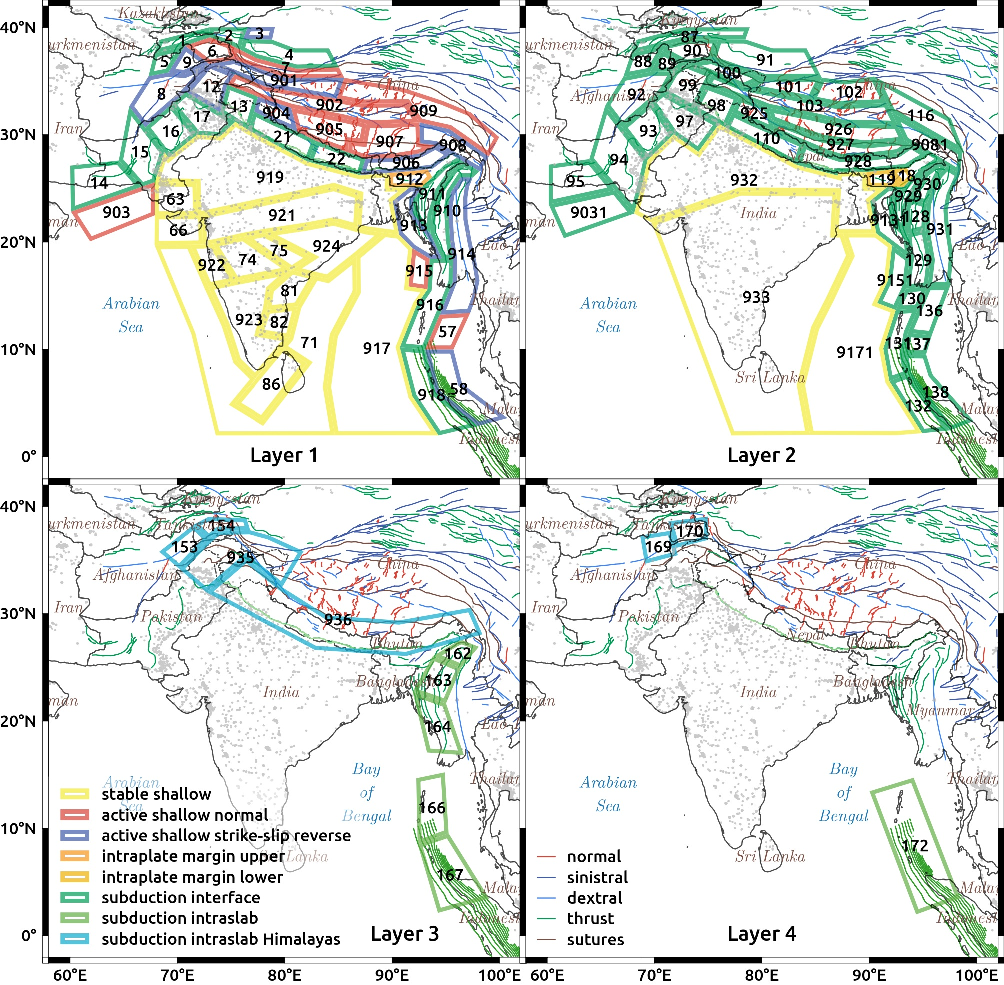
\includegraphics{India_Areal_Source_Model}
\end{adjustbox}
\caption[Areal source model]{Areal source model tectonic region assignments used in GMPE logic tree.
The areal source models is encoded in \texttt{\detokenize{areal_source_model.xml}}.
Zone identification numbers from \cite{nath2012probabilistic} are indicated.
Fault traces are from HimaTibetMap-1.0 \citep{styron2010database} except the Sumatran subduction fault which is from SLAB~1.0 \citep{hayes2012slab1}.
Fault data from the stable regions of India is lacking.
Urban areas, ``contiguous patches of built-up land greater than 1~km²'' \citep{schneider2009new}, are indicated in darker grey.}
\label{fig:ArealSourceModel}
\end{figure}

The lack of clear indications of how to assign various tectonic regions is a major shortcoming of the electronic supplement of \cite{nath2012probabilistic}. 
The tectonic region type assignments which were made for this study are summarized in \autoref{fig:ArealSourceModel}.
Among these assignments, the following could be problematic:
\begin{itemize}
\item Zone~17 at the edge of the Pamir ranges is arguably ``stable shallow crust'' but was assigned ``subduction interface''.
\item Zone~21 in the Himalayas has been assigned ``subduction interface'' because of the presence of the main Himalayan thrust fault. However events in this zone were included in \cite{sharma2009ground} and thus could possibly be modelled better using ``stable shallow crust strike-slip reverse''.
\item Zones~1, 2, 4, 5, 13--17, 22, 910 and 911 of layer 1 have been assigned ``subduction interface'' because of the presence of thrust faults but could arguably be better treated as part of ``stable shallow crust strike-slip reverse'' although events in these zones are not part of \cite{sharma2009ground}. Note that \cite{nath2011peak} only evaluated interface subduction models for events below 25 km depth.
\item Zone~906 in the Great Himalayas just north of the Shillong plateau was assigned ``active shallow crust strike-slip reverse'' even though the main Himalayan thrust runs through it, because the representative focal mechanism is strike-slip.
\item Zones~903 and 915-918 are predominantly oceanic crust but have been assigned ``active shallow crust'' or ``subduction interface'' according to the dominant focal mechanism and fault types.
For example zone~903 includes the Murray Ridge and so exhibits predominantly normal faulting as expected for a spreading ridge.
It is classified for the purpose of GMPE selection as ``active shallow crust normal'', but is likely in reality to produce ground motions distinct from an active continental crust.
\item Zones~71, 86 on layer~1 and zones 9031, 9081, 9131, 9151 and 9171 on layer~2 have have $a$ values of zero and so were assigned a ``no seismicity'' type and omitted from the areal source model.
\item Zones~169, 170 and 172 on layer~4 capture seismicity at 180-300~km depth, but only \cite{youngs1997strong} and \cite{kanno2006new} support depths below 180~km (see \autoref{table:GMPEs}).
\end{itemize}

Zones numbered as ``9xx'' in \cite{nath2012probabilistic} represent the amalgamation of several zones from \cite{thingbaijam2011seismogenic}.
In some cases this was done because of similarity of source mechanisms and statistics while in others it was necessary because the amount of seismicity in one of the zones was insufficient for FMD characterisation.
Furthermore, zones numbered ``9xx1'' in layer~2 have effectively had their seismicity transferred to the corresponding zones 9XX in layer~1.
For example zones 32 and 115 in \cite{thingbaijam2011seismogenic} become zones 908 and 9081 in \cite{nath2012probabilistic}, where zone~9081 has no seismicity.

Note that on layers 3 and 4 two distinct tectonic region types are defined for intraslab subduction \citep[p.
137]{nath2012probabilistic}.
Specifically, the ``Indo-Myanmar and Andaman-Sumatra subduction zones'' are assigned ``intraslab'' while the ``Himalayas and northwest India-Eurasia convergence'' are assigned ``intraslab Himalayas''.
Different GMPEs are applied in these regions, as described in \autoref{subsec:GmpeTree}, in particular the Japan and Cascadia adjustments of \cite{atkinson2003empirical} are applied, respectively.

Magnitude-scaling relations are used in PSHA to determine the actual rupture dimensions once a magnitude has been drawn from a frequency-magnitude distribution.
These were relatively straightforward to select once the tectonic region assignments were made, since ``\cite{wells1994new} for crustal events and those given by \cite{strasser2010scaling} for the subduction earthquakes'' \citep[p.~140]{nath2012probabilistic}.
It was inferred that for interface and intraslab regions \texttt{StrasserInterface} and \texttt{StrasserIntraslab} should be used, respectively.
The comment that ``the fault-rupture area estimated from the magnitude is constrained by a factor of 2'' \citep[p.~140]{nath2012probabilistic} was similarly interpreted as a width/depth aspect ratio of 2.

Since it is not explicitly stated in \cite{nath2012probabilistic} the seismogenic depth was assumed to be midway between the minimum and maximum for each layer.
Potential refinements to this setup are discussed in \autoref{app:SourceModelImprovements}.

The supplementary information required to generate the fully specified areal source model from the electronic supplement files \texttt{polygonlay\%d.txt} and \texttt{seismicitylay\%d.txt} files in the is contained in \texttt{auxiliary data.csv}.

\subsubsection{Smoothed-gridded points}
\label{subsubsec:Smoothed}

Smoothed-gridded seismicity models aim to replicate geographic variations of activity rates in a catalogue-driven way.
Typically a smoothing kernel is used which enforces a correlation distance and limits the resolution. The electronic supplement of \cite{nath2012probabilistic} includes smoothed-gridded values of $\nu$ for a set of latitudes and longitudes spanning the indian Subcontinent. Unfortunately neither the paper nor the data files themselves state whether $\nu$ is an annual activity rate, the total number of events, or something else.

After some discussion with K. Thingbaijam it was decided that although the models are described as ``spatially varying annual activity rates'' \cite[p.~140]{nath2012probabilistic} the electronic supplement actually contains spatially smoothed total seismicity, i.e. number of events (per cell).
In order to convert this information to activity rates, i.e. number of events per year (per cell), it was necessary to obtain the duration of each sub-catalogue.
Fortunately this missing ingredient is summarized in \cite[Table~1]{thingbaijam2011seismogenic} and reproduced in \autoref{table:Completeness}.

Given the total seismicity $N$ and the length in years of the relevant catalogue $T$ (see \autoref{table:Completeness}) the annual rate $\nu$ for a given model is obtained using:
\begin{equation} \label{eq:SeismicityToActivity} 
\nu = N/T 
\end{equation}

In OpenQuake-engine a smoothed-gridded seismicity model is handled as a set of point sources with specified frequency-magnitude distributions: at a minimum $a$, $b$ and $m_\text{max}$ must be specified.
\cite{nath2012probabilistic} indicate that ``$b$-value and $m_\text{max}$ remain fixed within the source zone''.
Thus in the present study for the smoothed seismicity model the parameters $b$ and $m_\text{max}$ of the truncated Gutenberg-Richter magnitude-frequency distributions are inferred from the areal source model zonation.
For points inside zones with non-zero $a$ values in the areal source model this is trivial; for points outside these zones the zone with the shortest perpendicular distance to the point was chosen.

\begin{figure}
\begin{adjustbox}{center}
\includegraphics{India_Smoothed_Source_Model}
\end{adjustbox}
\caption[Smoothed-gridded seismicity point source model]{Areal zone associations for smoothed-gridded seismicity point source model with $m_\text{min} = 4.5$.
While each point source has its own activity rate, other properties of the frequency-magnitude distribution, such as $b$ and $m_\text{max}$, and the tectonic subregion used for GMPE selection are taken from the associated areal zone.
Note that although the model is on a 0.1° grid, only the points on a 0.2° grid are plotted here.
Nominal smoothed seismicity source models are encoded in \texttt{\detokenize{smoothed_source_model_mmin4.5.xml}} and \texttt{\detokenize{smoothed_source_model_mmin5.5.xml}}}
\label{fig:SmoothedSourceModel}
\end{figure}

A gridded point source model also requires specification of  tectonic region type and source mechanism for the selection and implementation of GMPEs, as well as the uncertainty in the FMDs.
Thus the same procedure was used to assign tectonic subregion, rake, dip, strike, magnitude scaling relations, $\sigma_b$ and $\sigma_{m_\text{max}}$. For example the tectonic subregion assignments are shown for the smoothed-gridded model with $m_min$ = 4.5 in \autoref{fig:SmoothedSourceModel}.

The truncated Gutenberg-Richter magnitude-frequency distribution in OpenQuake-engine implements

$$ \lambda(M \geq m) = 10^{a - b m} = e^{\alpha - \beta m} $$

Ignoring events below some threshold $m_\text{min}$, the annual rate becomes

$$ \lambda(M \geq m_\text{min}) = e^{\alpha - \beta m_\text{min}} e^{-\beta (m - m_\text{min})} = \nu e^{-\beta (m - m_\text{min})} $$

Thus to compute the $a$ value for a point source from the activity rate $\nu$ for a given magnitude threshold, we take into account the $b$ value for the zone as follows:

$$a = \log_{10}(\nu) + b m_\text{min} $$

Similarly to compute the activity rate for an areal source we can use
\begin{equation} \label{eq:ArealActivity} 
\nu = 10^{a - b m_\text{min}}
\end{equation}

Since the data files for the smoothed seismicity models were neither clearly labeled nor described in detail in \cite{nath2012probabilistic} there was some doubt as to their proper interpretation. 
In order verify the assumptions made above it was decided to attempt to reconstruct the smoothed-gridded point source model from the events labeled as mainshocks in the original catalogue of \cite{nath2010earthquake}.
Some details of the smoothing are contained in the unpublished \cite{thingbaijam2011seismogenic}.
The smoothing methodology of \citet{frankel1995mapping} was used.
The years over which the catalogue was treated as complete are given (see \autoref{table:Completeness} and \autoref{app:Catalogue}). 
The smoothing kernel was Gaussian, with correlation distances of 65 and 85~km for $m_\text{min}$ of 4.5 and 5.5 respectively.

\autoref{fig:SmoothedReconstructed} shows the original and reconstructed gridded-smoothed seismicity models. 
The recomputed model was obtained using the implementation of \citet{frankel1995mapping} in the OpenQuake Hazard Modeller’s Toolkit \citep{weatherill2014openquake}.
Isotropic Gaussian smoothing kernels were used with correlation distances as as described above.
The correspondence is good but not perfect.

\begin{figure}
\begin{adjustbox}{center}
\includegraphics{Smoothed_Recalculated}
\end{adjustbox}
\caption[Original and reconstructed smoothed-gridded seismicity models]{%
Smoothed-gridded annual seismicity rates for layer 1 and $m_\text{min} = 4.5$. 
Original model of  \citet{nath2012probabilistic} is on left, while on the right is a model reconstructed from the catalogue of \cite{nath2010earthquake}.}
\label{fig:SmoothedReconstructed}
\end{figure}

Discrepancies between the original and reconstructed models can arise in many ways.
One possibility is different handling of catalogue events with unspecified depths (they were assumed to be in the shallowest layer) and depths below layer 4 (they were assumed to be in layer 4).
Doubts are raised as to the quality of declustering in \autoref{app:Catalogue}; it may be that the events labeled as ``mainshocks'' in \cite{nath2010earthquake} were not the ones used by \cite{thingbaijam2011seismogenic}.
Edge effects may be important in that the geographic limits of the catalogue and smoothed-gridded model are not identical.
In any case the reconstructed model shown was trimmed to contain only points specified in the original model.
Finally, it may be that the completeness intervals and correlation distances given in the preiminary study of \cite{thingbaijam2011seismogenic} were not those used in the final work of \cite{nath2012probabilistic}.
The correspondence is not perfect, but good enough to validate the assumptions made as to the interpretation of the electronic supplement data.

In order to verify that the smoothed and areal models are approximately equivalent to each other and the catalogue, annual activity rates were computed for each.
Areal activity rates were computed using \eqref{eq:ArealActivity}.
Smoothed model activity rates were computed by summing the seismicity for all points and then applying \eqref{eq:SeismicityToActivity}.
Catalogue activity rates were computed by querying the catalogue of \cite{nath2010earthquake} with appropriate minimum magnitudes and within the bounds of the areal source model.
Note also that events are only counted if the epicentre is within one of the zones of the areal model.
This was done on a layer-by-layer basis as well as over the whole model.

\begin{table}
\caption[Comparison of annual seismicity rates]{Comparison of annual seismicity rates for areal model, smoothed-gridded seismicity model and catalogue.
In each case the value shown is the average or expected number of events per year $\nu$ above the given minimum magnitude.
Catalogue events and smoothed-gridded point sources are only counted if the epicentre is within one of the zones of the areal model.}
\label{table:Rates}
\centering
\begin{tabular}{ccccccc}
\toprule
$m_\text{min}$ & \multicolumn{3}{c}{4.5} & \multicolumn{3}{c}{5.5} \\
source &  areal & smoothed & catalogue & areal & smoothed & catalogue \\
\midrule
layer   &      &        &         &       &          &           \\
1       &   80 &    130 &      54 &   8.4 &      4.1 &       3.1 \\
2       &   68 &    174 &      78 &  10.4 &      3.6 &       3.8 \\
3       &   36 &     89 &      40 &   2.9 &      1.7 &       1.6 \\
4       &   12 &     43 &      10 &   1.6 &      1.2 &       1.2 \\
total   &  194 &    435 &     182 &  23.3 &     10.6 &       9.7 \\
\bottomrule
\end{tabular}
\end{table}

The results are tabulated in \autoref{table:Rates}.
Both the areal and smoothed models tend to overestimate the seismicity in the catalogue.
Discrepancies between the areal model and the catalogue are likely an artefact of taking the total seismicity for a given zone, computing a frequency-magnitude distribution, and applying that FMD uniformly over the zone.
Discrepancies between the smoothed model and the catalogue cannot be explained by the smearing effect of the smoothing kernel, because this should result in smoothed seismicity rates lower than the catalogue rates when computed over the same area, whereas we observe smoothed seismicity rates which are higher.

Improvements to the smoothed seismicity model are proposed in \autoref{app:SourceModelImprovements}.

Other issues of note:
\begin{itemize}
\item Zones~9031, 9081, 9131, 9151 and 9171 on layer~2 have $m_\text{max}$ values values of zero.
These zones all the smoothed seismicity points in or nearest to these zones on layer~2 were assigned the $m_\text{max}$ values from the corresponding zones on layer~1, namely zones 903, 908, 913, 915 and 917.
\item Given that the Japan/Cascadia regional adjustments are used for intraslab subduction, it is not clear why they are not also applicable for interface subduction.
\item Although the hazard maps in the electronic supplement are at 0.2° and the paper says the smoothed-gridded models are also at 0.2° they are in fact at 0.1°.
\autoref{fig:SmoothedSourceModel} shows the model at just 0.2° for convenience.
\end{itemize}

\subsection{Ground-motion prediction equations}
\label{subsec:GMPEs}

In order to evaluate seismic hazard across the Indian subcontinent it is necessary to consider a wide range of tectonic and crustal propagation regimes, including some which may be unique to the region. 
In all, \cite{nath2012probabilistic} uses 21 GMPEs from 17 references, summarized in \autoref{table:GMPEs}. 

\afterpage{\clearpage\newgeometry{margin=2cm} 
\begin{landscape}
\begin{table}
\caption[Ground motion prediction equations]{Ground motion prediction equations used in this study.
``N'' indicates that models were newly implemented in OpenQuake for the current study.
``S'' indicates that the model has since been superseded by an equivalent model from the same authors.
Among the databases used, ``ENA'' stands for eastern North America, and ``NGA'' stands for next generation attenuation.
The tectonic region ``Type'' uses the following abbreviations: ``active'' shallow crust, ``intraplate'' margin, ``stable'' continental crust, ``interface'' subduction and ``intraslab'' subduction.
$N_E$ and $N_R$ are the number of earthquakes and records in the database, respectively.
$H$, $M$ and $R$ are the ranges of depth, magnitude and distance over which the GMPE is considered by the authors to be valid. The component ``C'' for which the GMPE is defined can be ``H'' for unspecified horizontal, ``R'' for random horizontal, ``A'' for average of horizontals, ``M'' for median of horizontals ``G'' for geometric mean of horizontals rotated into most adverse (GMRotI50) \citep{boore2006orientation}, ``S'' for peak of square root of sum of squares of horizontals or ``V'' for vertical.}
\label{table:GMPEs}
\centering
\begin{adjustbox}{center=\pagewidth}
\begin{tabular}{llcc >{\centering\arraybackslash}m{20mm} >{\centering\arraybackslash}m{15mm} ccccccccc}
\toprule
OpenQuake class & Reference & N & S & Database & 
Type & $N_E$ & $N_R$ & \multicolumn{2}{c}{$H$ [km]} & \multicolumn{2}{c}{$M$} &  \multicolumn{2}{c}{$R$ [km]} & C \\
\midrule
\texttt{ToroEtAl2002} & \cite{toro2002modification} & & & 
ENA & stable & \multicolumn{2}{c}{simulation} &
   &    & 5.0 & 8.0 &    & 1000 & A \\
\texttt{Campbell2003} & \cite{campbell2003prediction} & & & 
ENA & stable & \multicolumn{2}{c}{hybrid} &
   &     & 5.0 & 8.2 &  0 & 1000 & A \\
\texttt{AtkinsonBoore2006} & \cite{atkinson2006earthquake} & & & 
ENA & stable & \multicolumn{2}{c}{simulation} &
 2 &  30 & 5.0 & 8.3 &    & 1000 & H \\
\texttt{RaghukanthIyengar2007} & \cite{raghukanth2007estimation} & \checkmark & & 
peninsular India & stable & \multicolumn{2}{c}{simulation} &
 5 &  15 & 4.0 & 8.0 &    &  300 & A \\
\texttt{BooreAtkinson2008} & \cite{boore2008ground} & & \checkmark & 
NGA-West1 & active & 58 & 1574 &
   &     & 5.0 & 8.0 &  0 &  200 & G \\
\texttt{CampbellBozorgnia2008} & \cite{campbell2008nga} & &  \checkmark & 
NGA-West1 & active & 72 & 942 &
   &     & 4.0 & 8.0 &  0 &  200 & G \\
\texttt{SharmaEtAl2009} & \cite{sharma2009ground} & \checkmark & & 
Himalayas \& Zagros & active & 16 & 201 &
   &     & 5.0 & 7.0 &    &  100 & A \\
\texttt{AkkarBommer2010} & \cite{akkar2010empirical} & & \checkmark & 
Europe \& Middle East & active & 131 & 532 &
   &     & 5.0 & 7.6 &  0 &  100 & A \\
\texttt{NathEtAl2012Upper} & \multirow{2}{*}{\cite{nath2012ground}} & \checkmark & & 
Shillong & intraplate & \multicolumn{2}{c}{\multirow{2}{*}{simulation}} &
 0 &  25 & 4.8 & 7.6 & \multirow{2}{*}{10} &  \multirow{2}{*}{100} & \multirow{2}{*}{V} \\
\texttt{NathEtAl2012Lower} & & \checkmark & & plateau & margin & & &
25 &  40 & 4.8 & 8.1 &    &      &   \\
\texttt{AtkinsonBoore2003SInter} & \cite{atkinson2003empirical} & & & 
global & interface & 80 & 1155 &
20 &  50 & 5.0 & 8.3 & 10 &  550 & R \\
\texttt{ZhaoEtAl2006SInter} & \cite{zhao2006attenuation} & & \checkmark & 
Japan & interface & 269 & 1520 &
25 &  50 & 5.0 & 8.3 &    &  300 & A \\
\texttt{AtkinsonMacias2009} & \cite{atkinson2009predicted} & & & 
Cascadia & interface & \multicolumn{2}{c}{simulation} &
   &     & 7.5 & 9.0 &    &  400 & R \\
\texttt{Kanno2006Shallow} & \cite{kanno2006new} &  \checkmark & & 
Japan & active \textit{or} interface &  83 & 3769 &
 0 &  30 & 5.5 & 8.2 &    &  450 & S \\
\texttt{Kanno2006Deep} & \cite{kanno2006new} & \checkmark & & 
Japan & intraslab & 111 & 8150 &
30 & 200 & 5.5 & 8.2 &    &  450 & S \\
\texttt{YoungsEtAl1997SSlab} & \cite{youngs1997strong} & & & 
global & intraslab & 164 & 480 &
50 & 229 & 5.0 & 7.8 & 10 &  500 & A \\
\multicell{l}{\texttt{AtkinsonBoore2003SSlabJapan}\\\texttt{AtkinsonBoore2003SSlabCascadia}} & \cite{atkinson2003empirical} & \checkmark & & 
global &  intraslab &                80 & 1155 &
50 & 100 & 5.0 & 8.3 & 30 &  550 & R \\
\texttt{ZhaoEtAl2006SSlab} & \cite{zhao2006attenuation} & & \checkmark &
Japan & intraslab & 269 & 1725 &
50 & 120 & 5.0 & 8.3 &    &  300 & A \\
\texttt{LinLee2008SSlab} & \cite{lin2008ground} & & & 
Northeast Taiwan & intraslab & 54 & 4823 &
39 & 161 & 4.1 & 6.7 & 40 &  600 & A \\
\texttt{Gupta2010SSlab} & \cite{gupta2010response} & \checkmark & & 
Indoburman Arc & intraslab & 3 & 56 &
91 & 148 & 6.3 & 7.2 &    &  375 & M \\
\bottomrule
\end{tabular}
\end{adjustbox}
\end{table}
\end{landscape}
\restoregeometry\clearpage}

Nine of these GMPEs were new to OpenQuake-engine. 
These were implemented following the quality assurance procedures described in \cite{pagani2014openquake}. 
In this section the focus is on the necessity and appropriateness of these new GMPEs, as well as concerns which arose during their implementation.

In the process of the development of a GMPE specific to the Indian Himalayas, an area of rapid urbanization and elevated hazard \citep{sharma2009ground} excluded shallow India-Bangladesh and deep India-Burma border events from their database on the basis that PGA has different distance scaling.
This observation points to the necessity of different GMPEs for these types of events, in the former case a GMPE specific to the Shillong plateau \citep{nath2012ground} and in the latter case, one specific to Indoburman subduction \citep{gupta2010response}.

The Shillong plateau (zones 118 and 912 in \autoref{fig:ArealSourceModel}) is an example of a tectonic regime specific to India. 
Situated in between the Himalayan and Indoburman subduction zones it would be considered a stable crustal region were it not for the massive normal faulting events known to occur there.
The great Assam earthquake of 1897 destroyed buildings within several hundred~km.
The two main structures involved, the Dauki and Oldham faults, are capable of M > 8 plateau-building events with a recurrence interval of 3-8 kyr each \citep{bilham2001plateau}.
\cite{nath2012ground} notes stress drop apparently increasing with depth and models $\kappa$ using a database of recent and minor but well-recorded earthquakes, and uses this information to develop stochastic models for events in the upper and lower crust.
The simulations are of vertical rather than horizontal motion at a hard-rock site.

The GMPE of \cite{sharma2009ground} is intended for the Indian Himalayas but is based on data from both Zagros Mountains in Iran and the Himalayas.
The database included only a small number of events (see \autoref{table:GMPEs}), of which only a few were in the Himalayas, and none a result of normal faulting. 
Compared to the other models available for active regions it is the only one based on data from India.
It is furthermore a valuable addition to a logic tree in the Shillong plateau because unlike the other models available for that region, it is not based on stochastic simulation. The GMPE lacks a $M^2$ term and so \cite{cotton2006criteria} would counsel against its inclusion in a logic tree, but it is retained for lack of an alternative for the region. 
During implementation it was observed that it does not actually define coefficients for PGA so they were assumed to be the same as for the spectral acceleration at 0.04 s.

The GMPE of \cite{gupta2010response} is essentially a regionalization of \cite{atkinson2003empirical} for intraslab subduction. 
On the basis of a database of just three events, the constant term of \cite{atkinson2003empirical} was recalculated, leaving the distance, depth, magnitude and site amplification terms unchanged.

The GMPE of \cite{raghukanth2007estimation} was developed for the stable shallow crust of peninsular India using stochastic simulation.  
\cite{raghukanth2007estimation} actually describe three models based on regional variations in Q, for Koyna-Warna, southern India and western-central India, plus a model for all of peninsular India obtained by sampling the regional models in proportion to their landmass. 
It has been assumed that \cite{nath2012probabilistic} did not use the regional models. 
In implementing \cite{raghukanth2007estimation} typographical errors were identified in the coefficient Tables 2, 3 and 5 by comparing results obtained with the smoother published curves in Figures 3 and 5. 
The grossest error in Table~2(b) was fixed while 3 other errors causing a maximum error of approximately 10\% error were not fixed (see \url{ http://docs.openquake.org/oq-hazardlib/master/gsim/raghukanth_iyengar_2007.html}).

\cite{kanno2006new} specifies two models, for shallow and deep events, based on data predominantly from Japan. 
Rather than distinguishing between seismotectonic regimes, this GMPE gives appropriate scaling relations based on depth alone. 
Thus ``both crustal and subduction interface events fall into the category of shallow events'' (p. 883) where ``shallow'' is defined as a ``focal depth of 30~km or less'' (p. 883).
This flexibility allows the GMPE to be used for many tectonic regimes, although as discussed in \autoref{app:AlternativeGmpes} it should in future work be restricted to regions where it demonstrates good efficacy. 

\autoref{table:GMPEs} shows that layer~4 (180-300~km) is significantly deeper than deepest events used in regression for \citet[100~km]{atkinson2003empirical}, \citet[161~km]{lin2008ground}, \citet[120~km]{zhao2006attenuation} and \citet[148~km]{gupta2010response}. 
Of the GMPEs used for interface subduction in layer~4 only \citet[229~km]{youngs1997strong} includes events in the correct depth range.
In future work it would be beneficial to identify GMPEs appropriate for use in the depth range of layer~4 (see \autoref{app:AlternativeGmpes}.

Oddly, \cite{kanno2006new} is specified to 200~km depth, but is only used for interface events (layer~2).
Given the poor efficacy of \cite{kanno2006new} in the Hidukush/Pamirs it makes sense that it should be omitted in the Himalayas, but not in the Indo-Myanmar subduction zone.

It should be noted, finally, that \cite{kanno2006new} is defined for the ``peak square root of the sum of squares of two orthogonal horizontal components in the time domain'' (p. 880). Since the peak value is taken after computing the vectorial sum of the horizontals this is different from the (similarly rare) ``vectorial addition'' of \cite{douglas2003earthquake} where the sum is taken after  peak values are located in the time domain. 
This ground motion intensity measure component is more conservative than choosing a random horizontal component or the average of the peak horizontal components, but it is less conservative than the aforementioned vectorial addition. 
\autoref{table:GMPEs} shows that GMPEs for many different ground motion components are mixed in \cite{nath2012probabilistic}; this practice is not unusual but if left uncorrected errors do propagate through to hazard curves, and the resulting aleatory uncertainty is under-estimated \citep{beyer2006relationships}. 
OpenQuake tracks the type of horizontal component measured in its base \texttt{GroundShakingIntensityModel} class, but  does not currently make the necessary corrections to the mean or standard deviation of the ground motion.

\subsection{Source model logic tree}
\label{subsec:SourceTree}

\cite{nath2012probabilistic} accounts for the epistemic uncertainty in seismicity model parameters by estimating the standard deviations of $b$ and $m_\text{max}$ in each source zone and assigning weights to ±1 standard deviation for each source.

In reviewing the data, it was observed that \texttt{seismicitylay2.txt} listed standard deviation of $b$ in zone~93 as 0.9, and this results in an absurd amount of variability in the FMD for this zone. The rest of the standard deviations for $b$ vary from 0.03 to 0.16. It was decided that this must be a simple typographical error, and that the intended value must have been 0.09 instead. 

The source modelling part of the logic tree of \citet[Figure~4]{nath2012probabilistic} is shown in \autoref{fig:SourceTreeSymbolic}. 

\begin{figure}
\begin{adjustbox}{center}
\includegraphics{source_model_logic_tree_symbolic}
\end{adjustbox}
\caption[Symbolic source model logic tree]{Symbolic source model logic tree of \cite{nath2012probabilistic}.}
\label{fig:SourceTreeSymbolic}
\end{figure}

Note that although Figure~4 of \cite{nath2012probabilistic} shows the activity rate $\nu$ (and by implication $a$) varying with $b$. No values for the standard deviation of $a$ or $\nu$ are provided in the electronic supplement of \cite{thingbaijam2011seismogenic}, thus it was assumed that the intent is to recalculate $a$ whenever $b$ is varied in order to maintain constant total moment rate.
This is the default behaviour in OpenQuake-engine when using the uncertainty type \texttt{bGRRelative}.

\subsubsection{Full or partial enumeration}
\label{subsubsec:Enumeration}

\autoref{fig:SourceTreeSymbolic} is the source model logic tree in \textit{symbolic} form.
If this is actually expanded to encompass all source zones the result is a source model logic tree far too large to represent on a page; just a portion of it is shown in \autoref{fig:SourceTreePartial}.

\begin{figure}
\begin{adjustbox}{center}
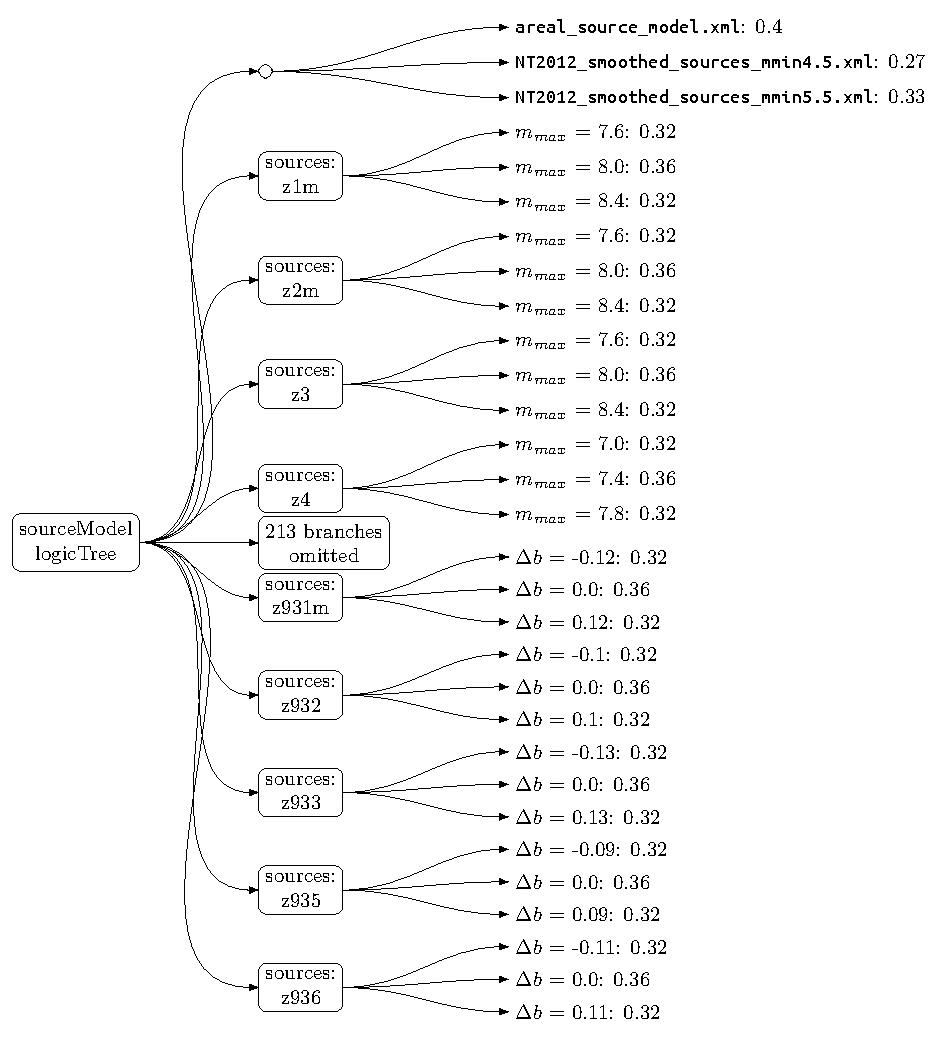
\includegraphics{source_model_logic_tree}
\end{adjustbox}
\caption[Partial source model logic tree]{Partial source model logic tree of \cite{nath2012probabilistic}.
The full model is encoded in \texttt{\detokenize{source_model_logic_tree.xml}}}
\label{fig:SourceTreePartial}
\end{figure}

The fact that \autoref{fig:SourceTreePartial} has to be truncated is not simply a lack of page space.
Although it is common practice to diagram logic trees in parallel, full enumeration of such logic trees actually takes place in series.
Thus, rather than just $3\times223$ branches there are in fact $3^{223} \approx 10^{106}$ (i.e. approximately one million googol) terminal branches implied in a full enumeration of \autoref{fig:SourceTreePartial}.
Full enumeration of the logic tree is clearly out of the question.
It may even be computationally prohibitive simply to calculate the weights on the terminal branches, a necessary precursor to partial enumeration by Monte Carlo sampling.
(In any case it was not possible to complete even an analysis by partial enumeration on the current version of OpenQuake.)

Given that sources are only considered when located within a certain radius of any given site \citep[200 km]{nath2012probabilistic}, an algorithm could be developed to find all subsets of the sites with a common subset of sources within that radius.
Of the cities listed in \citet[Table~3]{nath2012probabilistic}, Shillong and Imphal have the most zones within a 200 km radius, at 14, and Guwahati is next at 12.
If for each site only the nearest 14 zones are considered, then the symbolic logic tree of \autoref{fig:SourceTreeSymbolic} expands to a more tractable $3^{29} \approx 7\times10^{13}$ branches.
For a mapping application where many sites are located on a grid those sites could be sorted into groups of sites having common contributing source zones; each group would then have a distinct set of logic tree realizations to enumerate or be sampled from.
The scheme described above is effectively a means of generating a logic tree without its geographically irrelevant branches (n.b. not ``pruning'' which implies branch exists before it is removed).
This mode of logic tree enumeration is not currently available in OpenQuake nor is it mentioned in \cite{nath2012probabilistic}. 

Note when a source model consists of a grid of point sources, it is neither possible nor advisable to try to apply full enumeration of a symbolic logic tree such as \autoref{fig:SourceTreeSymbolic}.
It is not possible because when the number of sources is on the order of 400000, as the case of \cite{nath2012probabilistic}, the number of terminal branches is not even representable as a 64-bit float.
It is not advisable because if it makes sense to vary $b$ and $m_\text{max}$ at all it is because these properties vary on a sub-regional scale.
For example an $m_\text{max}$ exists because of the actual physical sizes of the faults, and a $b$ value exists because of stress regimes.
Using the site grouping and distance limit as described above it should be possible to fully enumerate a smoothed-gridded source model, as long as the variability $b$ and $m_\text{max}$ is applied only on groups of point sources, the most natural grouping being one devised according to an areal source model.

Given the above discussion, it is unlikely that \cite{nath2012probabilistic} performed full or even partial enumeration of their model of source uncertainty.

Another possibility is that they applied the positive and negative deviations to the mean values of $b$ and $m_\text{max}$ for all areal and point sources simultaneously.
In this case there would be a very manageable number of terminal branches, $3^2$ = 27, each with a different FMD for every zone. 
This possibility must be dismissed as grossly over-weighting the possibility, for example, that all sources jointly have the highest possible $m_\text{max}$ and lowest possible $b$.

\cite{nath2012probabilistic} only publish mean hazard curves and maps.
Nowhere are median or quantile hazards discussed; effectively there is no discussion of the effect of aleatory and epistemic uncertainty in the models on the uncertainty of the results.

\subsubsection{Collapse of frequency-magnitude distributions}
\label{subsubsec:Collapse}

In classical PSHA the hazard integral gives an estimate of rate at which the ground motion $Y$ at a site of interest will exceed some value $y$. For a set of $N_S$ sources generating ruptures of $N_M$ magnitudes $m_j$ at $N_R$ distances $r_k$ using discrete summations \citep{baker2008introduction}:
\begin{equation} \label{eq:HazardRateSummation} 
\lambda(Y > y) = 
\sum_{i=1}^{N_S} 
\lambda(M_i > m_\text{min}) 
\sum_{j=1}^{N_M} 
\sum_{k=1}^{N_R} 
P_i(Y > y|m_j,r_k) 
P_i(M_i=m_j) 
P_i(R_i=r_k)
\end{equation}
where for source $i$:
\begin{itemize}
\item $\lambda_i(M_i > m_\text{min})$ is the rate of earthquakes greater than $m_\text{min}$
\item $P_i(Y > y|m_j,r_k)$ is the ground motion prediction equation (GMPE) and incorporates aleatory uncertainty in the ground motion
\item $P_i(M_i=m_j)$ is the frequency-magnitude distribution (FMD)
\item $P_i(R_i=r_k)$ is the distribution of distance measures from points within the source to the site of interest.
\end{itemize}

For a single point source, neglecting finite source effects, this simplifies to:
$$ 
\lambda(Y > y) = 
\lambda(M > m_\text{min}) 
\sum_{j=1}^{N_M} 
P(Y > y|m_j,R) 
P(M=m_j) 
$$

Now suppose that certain epistemic uncertainties have been identified. 
In order to estimate the effect of this lack of knowledge on the distribution of ground motions suppose $N_G$ GMPEs $P_\ell(Y > y|m_j,R)$ have been assigned weights $w_\ell$ and $N_F$ FMDs $P_m(M=m_j)$ have been assigned weights $w_m$. 
This is accomplished via
$$ 
\lambda(Y > y) = 
\lambda(M > m_\text{min}) 
\sum_{m=1}^{N_F} w_m 
\sum_{\ell=1}^{N_G} w_\ell 
\sum_{j=1}^{N_M} 
P_\ell(Y > y|m_j,R) 
P_m(M=m_j) 
$$
but we can reorder the summations to obtain
$$ 
\lambda(Y > y) = 
\lambda(M > m_\text{min}) 
\sum_{\ell=1}^{N_G} w_\ell 
\sum_{j=1}^{N_M} 
P_\ell(Y > y|m_j,R) 
\sum_{m=1}^{N_F} w_m 
P_m(M=m_j) 
$$

By pre-computing the ``collapsed'' FMD for the source
$$ 
P_C(M=m) \triangleq 
\sum_{m=1}^{N_F} w_m P_m(M=m) 
$$
we can simplify the hazard summation to
$$ 
\lambda(Y > y) = 
\lambda(M > m_\text{min}) 
\sum_{\ell=1}^{N_G} w_\ell 
\sum_{j=1}^{N_M} 
P_\ell(Y > y|m_j,R) 
P_C(M=m_j) 
$$

At this point it is critical to note that a further ``collapse'' of GMPE uncertainty is not possible because the ground motion is conditional upon the magnitude.

Returning to the case of multiple sources in \eqref{eq:HazardRateSummation}, we can include ground-motion and frequency-magnitude epistemic uncertainty by writing
$$ \lambda(Y > y) = 
\sum_{i=1}^{N_S} 
\lambda_i(M_i > m_\text{min}) 
\sum_{m=1}^{N_F} w_{mi} 
\sum_{\ell=1}^{N_G} w_{\ell,i}
\sum_{j=1}^{N_M} 
\sum_{k=1}^{N_R} 
P_{\ell i}(Y > y|m_j,r_k) 
P_{mi}(M_i=m_j) 
P_i(R_i=r_k) $$
and we can still reorder the summations, as long as we recognize that the collapsed FMD is different for each source
$$
\lambda(Y > y) = 
\sum_{i=1}^{N_S} 
\lambda(M_i > m_\text{min}) 
\sum_{\ell=1}^{N_G} w_{\ell i}
\sum_{j=1}^{N_M} 
\sum_{k=1}^{N_R} 
P_{\ell i}(Y > y|m_j,r_k) 
P_i(R_i=r_k) 
\sum_{m=1}^{N_F} w_{mi} 
P_{mi}(M_i=m_j) 
$$

Thus for a rate-based formulation we can pre-compute the collapsed FMD for each source
\begin{equation} \label{eq:CollapsedFmd} 
P_{Ci}(M_i = m) \triangleq
\sum_{m=1}^{N_F} w_{mi} 
P_{mi}(M_i=m) 
\end{equation}
And compute the mean hazard using
\begin{equation} \label{eq:RateHazardCollapsed} 
\lambda(Y > y) = 
\sum_{i=1}^{N_S} 
\lambda(M_i > m_\text{min}) 
\sum_{\ell=1}^{N_G} w_{\ell i}
\sum_{j=1}^{N_M} 
\sum_{k=1}^{N_R} 
P_{\ell i}(Y > y|m_j,r_k) 
P_i(R_i=r_k) 
P_{Ci}(M_i = m_j) 
\end{equation}

An example of the process of pre-computing collapsed FMDs as described in equation \eqref{eq:CollapsedFmd} is shown in \autoref{fig:CollapsedFmd}.

\begin{figure}
\begin{adjustbox}{center}
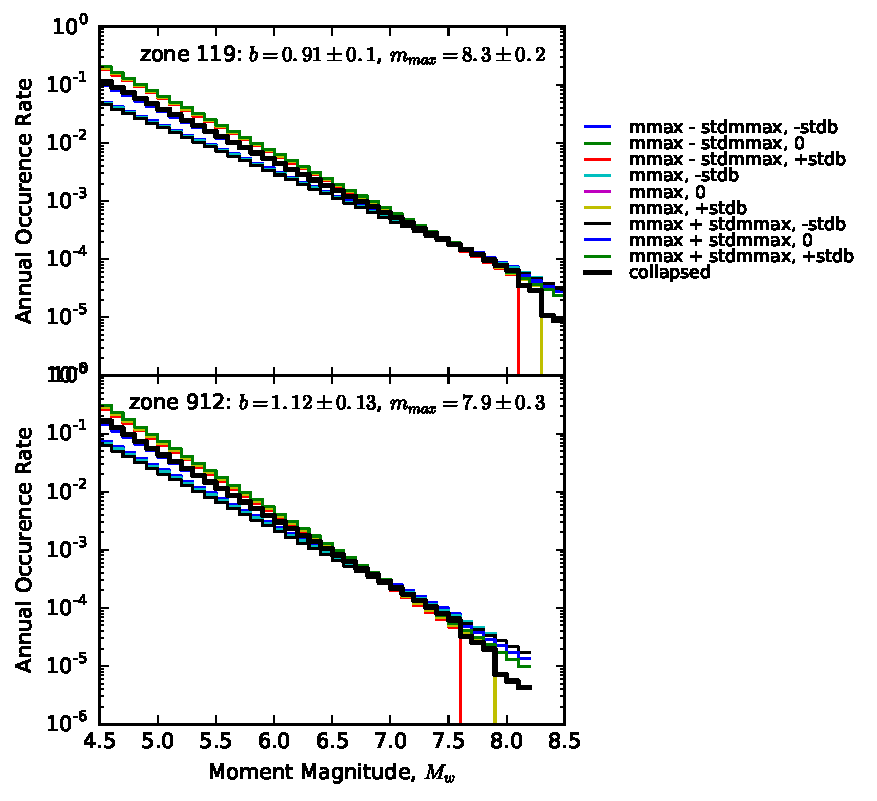
\includegraphics{Mean_Occurrence_Rates_Zones_119_912}
\end{adjustbox}
\caption[Frequency-magnitude distributions for two zones nearest to Guwahati, India]{Frequency-magnitude distributions corresponding to various branches of the logic tree of \cite{nath2012probabilistic}. 
The zones chosen are the two closest to Guwahati, India. 
Zone~119 at 25-50 km depth is the zone capable of producing a devastating ``pop-up'' type event \citep{Bilham2001, nath2012ground}. 
The ``collapsed'' FMD uncertainty computed using \eqref{eq:CollapsedFmd} is shown as a heavy black line.} 
\label{fig:CollapsedFmd}
\end{figure}

The preceding analysis shows that collapsed FMDs should give an exact result for the mean exceedance rate computed using a rate-based formulation. 
\autoref{fig:MeanFullVsCollapsed} shows that in practice using OpenQuake, the collapsing of FMDs gives a very good approximation of the mean hazard for low probabilities of exceedance but not for high. 
The difference is due to the fact that OpenQuake-engine computes PSHA not using the classical rate-based formulation but using the probability-based formulation of OpenSHA \citep{field2003opensha,pagani2014openquake}.
This issue will be revisited at the end of this section.

\begin{figure}
\begin{adjustbox}{center}
\includegraphics{Guwahati_mean_Zones_119_912_1year}
\end{adjustbox}
\caption[Mean hazard curves computed using various levels of FMD uncertainty]{Mean hazard curves computed using various levels of FMD uncertainty. 
The site of interest is the city of Guwahati. 
The source model consists only of zones 119 and 912 of \cite{nath2012probabilistic}. 
The full GMPE logic tree of \cite{nath2012probabilistic} is used. 
The ``fully enumerated'' result implements the FMD logic tree described in \cite{nath2012probabilistic} while ``collapsed'' implements \eqref{eq:CollapsedFmd} and ``no FMD uncertainty'' models only the FMD logic tree branches with the largest weights.} 
\label{fig:MeanFullVsCollapsed}
\end{figure}

The important point here is that the ``collapsed'' FMD can be pre-computed for each source. 
In an application with $N_S$ sources, if there are $3^2$ branches to the FMD logic tree this means $3^{2 N_S}$ branches can be eliminated in all. 
In a simple example with a single site, two areal sources and a moderately complex GMPE logic tree (see \autoref{fig:MeanFullVsCollapsed}) computation time on a quad-core laptop dropped from 36 minutes to 55 seconds when FMD uncertainty was collapsed. 
In mapping type applications with gridded sites and hundreds of areal sources, each with FMD uncertainty, the computational savings can make an intractable problem tractable. 

\begin{figure}
\begin{adjustbox}{center}
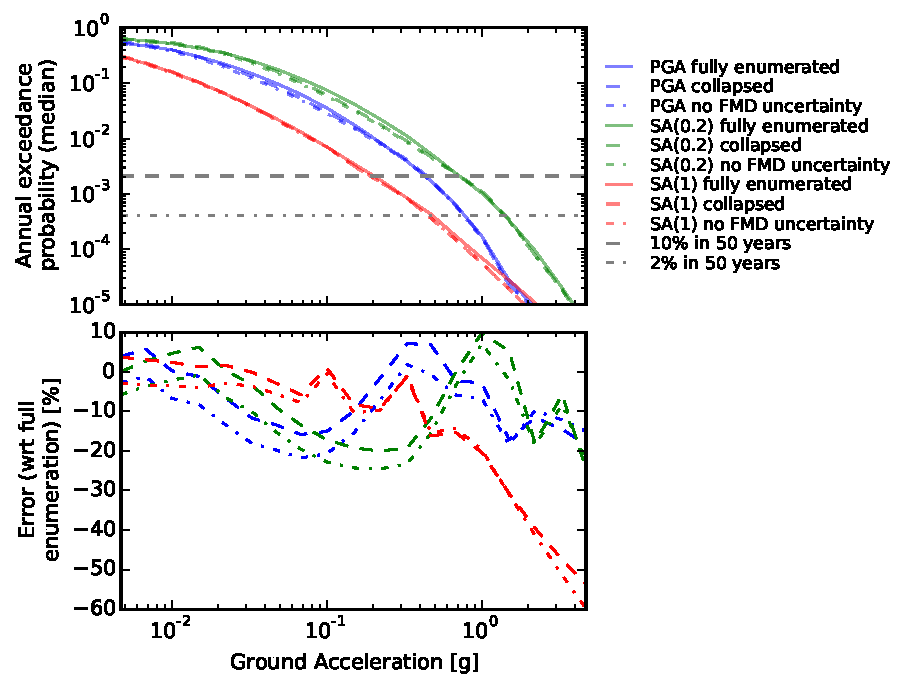
\includegraphics{Guwahati_median_Zones_119_912_1year}
\end{adjustbox}
\caption[Median hazard curves computed using various levels of FMD uncertainty]{Median hazard curves computed using various levels of FMD uncertainty. 
For detailed description see \autoref{fig:MeanFullVsCollapsed}.} 
\label{fig:MedianFullVsCollapsed}
\end{figure}

The hazard integral \eqref{eq:HazardRateSummation} only estimates the mean hazard, not the median or quantiles. 
Aleatory variability is modelled in most if not all GMPEs using a log-normal distribution so the ability to compute an arbitrary quantile of ground-motion exceedance is built-in. 

In OpenQuake, the effect of epistemic variability on quantiles is handled as follows.
First, as mentioned in \autoref{subsubsec:Enumeration}, terminal branches or ``realizations'' are enumerated, and  weights assigned to each. 
In some cases, with large numbers of sources, each having FMD uncertainty, OpenQuake-engine founders simply in enumerating realizations. 
For each realization and intensity measure type and level the probabilities of exceedance are computed. 
Finally, these probabilities are then sorted quantiles are located with reference to the weighting scheme. 
As a simplistic example, if there are 3 FMD branches for a source, then whichever produces the largest probability of exceedance at a given level of ground motion will determine the probability of exceedance for any percentile from the 67\textsuperscript{th} through the 100\textsuperscript{th}. 
Furthermore, if there are no other logic trees, for GMPEs or source models, then in fact the 67\textsuperscript{th} will be the same as the 100\textsuperscript{th} percentile hazard curve.

With the FMD logic trees collapsed the ground motions for different realizations are no longer computed and cannot be sorted, as required to find a quantile of interest. 
The result is just plain wrong, farther from the true result than if no FMD uncertainty is considered at all, as shown in \autoref{fig:MedianFullVsCollapsed}.
Given this understanding it is clear that ``collapse'' of FMDs cannot produce correct results for quantile hazard curves, or at least it cannot convey properly the part of the uncertainty due to epistemic uncertainty in the FMDs.

A slightly more general case than that given by \cite{baker2008introduction} is to treat the probability of an event at a given distance from a site as dependent on magnitude. In this case for a non-point source \citep[equation~A2]{field2003opensha}
$$ 
\lambda(Y > y) = 
\lambda(M > m_\text{min}) 
\sum_{j=1}^{N_M} 
\sum_{k=1}^{N_R} 
P(Y > y | m_j,r_k) 
P(R=r_k | m_j)
P(M=m_j) 
$$ 

To assess the effect of epistemic uncertainties on the mean we must compute
\begin{equation} \label{eq:NonPointPreCollapse} 
\lambda(Y > y) = 
\lambda(M > m_\text{min}) 
\sum_{m=1}^{N_F} w_m 
\sum_{\ell=1}^{N_G} w_\ell 
\sum_{j=1}^{N_M} 
\sum_{k=1}^{N_R} 
P_\ell(Y > y | m_j,r_k) 
P(R=r_k | m_j)
P_m(M=m_j) 
\end{equation} 
but in many cases it will be reasonable to treat the distribution of site-source distances as independent of the frequency-magnitude distributions, so that the summations can still be reordered  
$$ 
\lambda(Y > y) = 
\lambda(M > m_\text{min}) 
\sum_{\ell=1}^{N_G} w_\ell 
\sum_{j=1}^{N_M} 
\sum_{k=1}^{N_R} 
P_\ell(Y > y | m_j,r_k) 
P(R=r_k | m_j)
\sum_{m=1}^{N_F} w_m 
P_m(M=m_j) 
$$ 
and the FMDs can be collapsed.

The hazard for each source must then be summed to compute the hazard for a given site. There may be instances where uncertainty regarding $m_\text{max}$ is connected to uncertainty regarding the physical extent of a source. This sort of epistemic uncertainty would have to be handled differently, as weighted alternative source models.

Finally we return to the issue of the inaccuracy of the results obtained using OpenQuake at high probability of exceedance. 
The formulation of the hazard integral \eqref{eq:HazardRateSummation} implemented in OpenQuake-engine assumes a Poisson model for earthquake occurrence, and furthermore that the probability of two or more occurrences of each source is zero in the time interval of interest \citep{field2003opensha,pagani2014openquake}.
Rather than the rate of exceedance, the probability of exceedance in a given time interval is computed.
Similarly, rather than depending on the rate of events over a given minimum $\lambda(M > m_\text{min})$, it is written in terms of the probability of a single occurrence of an event (with a minimum magnitude) in a given time interval $P(\text{occur}_i)$.
Rewriting the formulation of \citet[equation~A9]{field2003opensha}:
$$ 
P(Y > y) = 
1 - \prod_{i=1}^{N_S} \left[
1 - \sum_{j=1}^{N_M} \sum_{k=1}^{N_R} 
P(\text{occur}_i) 
P(Y > y | m_{ij},r_{ijk}) 
P(R=r_{ijk} | m_{ij})
P(M=m_{ij}) \right]
$$ 
Whereas when working with rates epistemic uncertainty is treated by computing a weighted sum of predicted weights, with probabilities it is treated by computing one minus the product of the probabilities of non-occurrence.

The incorporation of epistemic uncertainty in the selection of GMPEs and FMDs is implemented in OpenQuake-engine by computing a weighted sum of probabilities (Graeme Weatherill, personal communication).
Neglecting the possibility of dependence of the distance distribution on magnitude, the summation is then:
$$ 
P(Y > y) = 
\sum_{m=1}^{N_F} w_m 
\sum_{\ell=1}^{N_G} w_\ell \left\{
1 - \prod_{i=1}^{N_S} \left[
1 - \sum_{j=1}^{N_M} \sum_{k=1}^{N_R} 
P(\text{occur}_i) 
P_\ell(Y > y | m_{ij},r_{ijk}) 
P(R=r_{ijk})
P_m(M=m_{ij}) \right] \right\}
$$ 

As long as the probability of exceedance for any given realization $m,\ell$ is much smaller than unity, the product can be rewritten as a summation by discarding higher-order terms. In this case we get
$$ 
P(Y > y) = 
\sum_{m=1}^{N_F} w_{mi} 
\sum_{\ell=1}^{N_G} w_{\ell i}
\sum_{i=1}^{N_S} 
\sum_{j=1}^{N_M} 
\sum_{k=1}^{N_R} 
P(\text{occur}_i) 
P_\ell(Y > y | m_{ij},r_{ijk}) 
P(R=r_{ijk})
P_m(M=m_{ij})
$$ 
and proceed as from \eqref{eq:NonPointPreCollapse} to arrive at
$$ 
P(Y > y) = 
\sum_{\ell=1}^{N_G} w_\ell 
\sum_{i=1}^{N_S} 
\sum_{j=1}^{N_M} 
\sum_{k=1}^{N_R} 
P(\text{occur}_i) 
P_\ell(Y > y | m_{ij},r_{ijk}) 
P(R=r_{ijk})
P_{Ci}(M_i = m_j)
$$ 
where the collapsed FMD for source $i$, $P_{Ci}(M_i = m_j)$ is computed as for the rate-based formulation using equation \eqref{eq:CollapsedFmd}

In conclusion, the collapse of FMD logic trees by weighted summation of branches is perfectly safe for the classical formulation of the hazard integral with handling of epistemic uncertainty by summation of rates. 
When mean hazard is computed using the OpenSHA formulation of \cite{field2003opensha} and epistemic uncertainty is handled by summation of probabilities, for example using OpenQuake, care must be taken that the probabilities of exceedance of the individual realizations are all small.
In many cases inaccuracy at low-probability of exceedance is effectively a computational artefact, a curiosity of no engineering significance.
It is always possible, however, to reduce the error without computational cost by reducing the investigation time.
For example, in the above example reducing the investigation time from 1~year to 1 month reduced the maximum error in the mean hazard from 3\% to 0.25\%.

This method gives a significant reduction in computational complexity, but can only be used to compute the mean hazard, not the median or quantiles. 
In many cases, such as the present one, an intractable problem become tractable.
In \autoref{sec:Results} the hazard results presented were obtained via the collapsing of FMD uncertainty.
In collapsing the FMD branches of the source model logic tree of \autoref{fig:SourceTreeSymbolic} these branches are effectively deleted, leaving only the branch set giving weights to the areal and smoothed source models.

\section{Hazard results}
\label{sec:Results}

Validation of PSHA results would require comparison against observed hazard. 
This in turn would require a catalogue many times longer than the significant return periods, something which won't be available for centuries.
In this work we are merely verifying that the current model gives result close to those of \cite{nath2012probabilistic}.

Results in this section were obtained using the model files in \autoref{app:Jobs} and OpenQuake Release~1.9.

\subsection{Verification}
\label{subsec:Verification}

The electronic supplement of \cite{nath2012probabilistic} contains probabilities of exceedance on an 0.2° grid of latitude and longitude for several intensity measures. 
Unfortunately this data does not correspond to the hazard maps shown in Figures~7 and S1 of \cite{nath2012probabilistic}, as shown in \autoref{fig:ElectronicSupplement}.

\begin{figure}
\begin{adjustbox}{center}
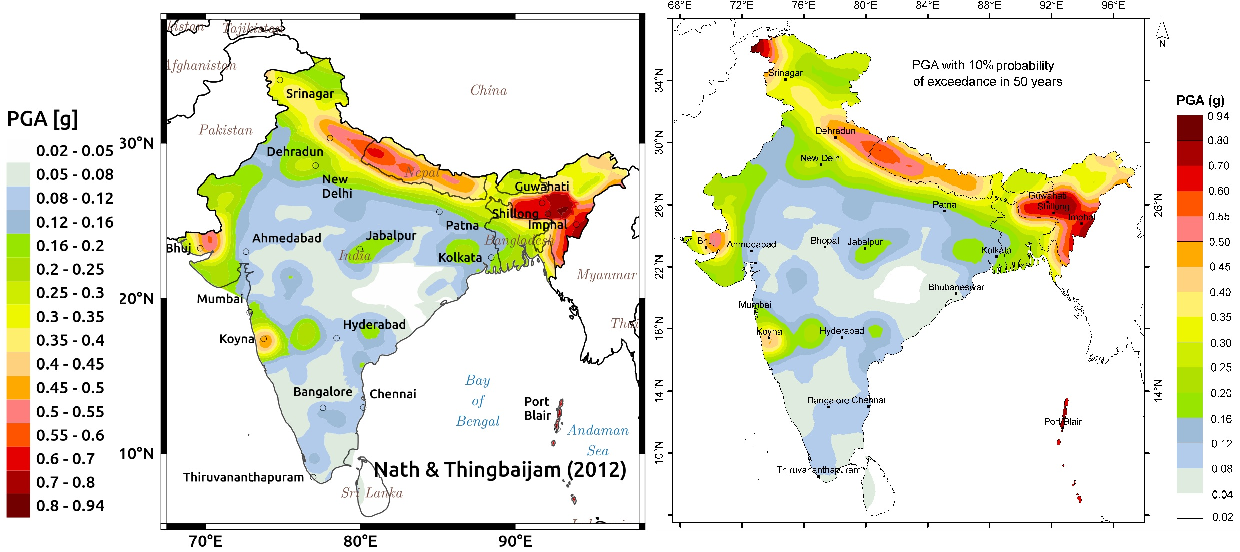
\includegraphics[width=1.2\textwidth]{electronic_supplement_contoured}
\end{adjustbox}
\caption[Comparison of original hazard maps in paper and electronic supplement]{
Comparison of original hazard maps for PGA with 10\% probability of exceedance (POE) in 50~years. 
On the right is Figure~S1 A from the electronic supplement, which is a colour version of the top left panel of Figure~7 in \cite{nath2012probabilistic}. 
On the left is data from the relevant column of \texttt{India\_pga.csv}, contoured using the Contour plugin version 1.3.5 of the QGIS software mapping package \citep{qgis2016user}.}
\label{fig:ElectronicSupplement}
\end{figure}

There are many points of dissimilarity between the published figures and data for hazard results.
One of the most confounding is the ``ridge'' of rapid change in PGA at about 22°N between 80°E and 85°E. 
The ridge does not correspond to the boundary of any areal source.
Similar features are seen in the data files for all intensity measures and probabilities of exceedance.
For these reasons the electronic supplement result data files are considered to be in error.
Future verification of hazard should be done exclusively against the published figures.

Unfortunately, due to the size of the model and problems with the current version of the OpenQuake-engine (Release 1.9) it has not been possible to generate a full hazard map.
For now we must content ourselves instead with verification of hazard at selected cities.

The current model is compared to Table~3 of \cite{nath2012probabilistic} in \autoref{table:CitiesHazard}. 
Similarly, the hazard curves in Figure~6 of \cite{nath2012probabilistic} are compared to the current study in \autoref{fig:CitiesHazard}.

\begin{table}
\caption[Mean PGA at 10\% POE in 50~years in selected cities]{
Mean PGA in selected cities. 
Cities are located on the map of \autoref{fig:ElectronicSupplement}.
`NT2012'' is the peak ground acceleration at 10\% probability of exceedance in 50~years from Table~3 of \cite{nath2012probabilistic}. 
``A2016'' is the same measure of hazard from the current study.
The error is that of A2016 relative to NT2012.}
\label{table:CitiesHazard}
\centering
\begin{tabular}{lcccccc}
\toprule
\multirow{2}{*}{City} 
                    & Latitude & Longitude & NT2012 &  A2016 & 
                                                  \multicolumn{2}{c}{Error} \\
                    &     [°N] &      [°E] &    [g] &    [g] &   [g] & [\%] \\
\midrule
           Srinagar &    34.08 &     74.80 &   0.33 &  0.417 &  0.09 &  26 \\
              Koyna &    17.40 &     73.75 &   0.47 &  0.455 & -0.02 &  -3 \\
          New Delhi &    28.56 &     77.11 &   0.24 &  0.232 & -0.01 &  -3 \\
             Imphal &    24.78 &     93.94 &   0.68 &  0.636 & -0.04 &  -6 \\
          Bangalore &    12.98 &     77.58 &   0.11 &  0.097 & -0.01 & -12 \\
           Guwahati &    26.18 &     91.73 &   0.66 &  0.562 & -0.10 & -15 \\
           Dehradun &    30.33 &     78.04 &   0.47 &  0.393 & -0.08 & -16 \\
         Port Blair &    11.61 &     92.72 &   0.71 &  0.583 & -0.13 & -18 \\
               Bhuj &    23.25 &     69.66 &   0.42 &  0.337 & -0.08 & -20 \\
           Shillong &    25.48 &     92.11 &   0.72 &  0.538 & -0.18 & -25 \\
            Chennai &    13.00 &     80.18 &   0.12 &  0.086 & -0.03 & -29 \\
             Mumbai &    19.11 &     72.85 &   0.16 &  0.110 & -0.05 & -31 \\
            Kolkata &    22.65 &     88.45 &   0.15 &  0.102 & -0.05 & -32 \\
          Hyderabad &    17.45 &     78.46 &   0.09 &  0.061 & -0.03 & -32 \\
              Patna &    25.60 &     85.10 &   0.13 &  0.085 & -0.04 & -35 \\
          Ahmedabad &    23.03 &     72.61 &   0.11 &  0.062 & -0.05 & -43 \\
 Thiruvananthapuram &     8.50 &     76.95 &   0.07 &  0.037 & -0.03 & -47 \\
           Jabalpur &    23.20 &     79.95 &   0.19 &  0.099 & -0.09 & -48 \\
\bottomrule
\end{tabular}
\end{table}

Expressed as a percentage \autoref{table:CitiesHazard} shows significant difference between current results and published values. 
At 10\% POE in 50~years there is a single site with PGA 26\% too high (Sringar) and many sites with PGA up to 48\% too low. 
However, there is a trend to larger error where the hazard was lower. 
It turns out the absolute error is never greater than 0.18~g, and among the cities with high hazard the error is never greater than ±26\%.

\begin{figure}
\begin{adjustbox}{center}
\includegraphics{Figure_6_Reproduced}
\end{adjustbox}
\caption[Mean hazard curves for selected cities]{%
Mean hazard curves for selected cities.
Solid lines are the results of the current study.
Dashed lines results digitized from Figure~6 of \cite{nath2012probabilistic}.}
\label{fig:CitiesHazard}
\end{figure}

\autoref{fig:CitiesHazard} shows that in the cities with highest hazard (e.g. Bhuj, Guwahati, Koyna and New Delhi) the current model gives lower hazard at low probability of exceedance and higher hazard at high probability of exceedance.
In other cities, those with lower hazard, the current model gives lower hazard at all probabilities.

\subsection{Discussion}
\label{subsec:Discussion}

Although better agreement was hoped for, agreement within ±26\% in the cities with high hazard is a good result for the first revision of the new model, especially given the incomplete documentation of the reference model. 

More work is needed to determine where the remaining discrepancies lie.
First it will be important to plot the hazard map for the new model, and particularly the difference between the new map and the reference map.
This will give a sense of exactly how the error is regionalized.
For example, the remaining error may be associated with one or more zones or tectonic region types, or it may track the peaks of the smoothed seismicity model.

A hazard error map such as those used to compare 2008 and 2014 models in \cite{petersen2014documentation} would be quite diagnostic; without it we can really only speculate as to likely sources of discrepancies.

One possibility is that the subduction interface tectonic region types should not be used in layer 1 because \cite{nath2011peak} only evaluated interface subduction GMPEs for events below 25 km depth. 
It may not be correct to use GMPEs for active shallow crust where subduction faults come to the surface, but at the outset we are just trying to reproduce the results of \cite{nath2012probabilistic}. 
There could in fact be many more incorrectly assigned tectonic region types; it should be possible to locate and correct these as well using a hazard error map.

Another possibility is that the smoothed seismicity model files could still be being interpreted incorrectly.
In this case switching to regenerated smoothed seismicity models as discussed in \autoref{app:Catalogue} will bring us no closer to verification.

It is possible that no correspondence between hazard map errors and areal or smoothed seismicity models will be observed. 
The conclusion would be that the rupture forecast (i.e. distributions of rupture areas and hypocenters) generated by OpenQuake is significantly different from the closed-source software of \cite{nath2012probabilistic}.
In this case there is nothing we can do to better verify the model, but at the same time there would be nothing wrong with it and it could safely be used as the basis for future work.

A final comment.
\cite{bommer2008use} notes that ``PSHA should always be done together with a disaggregation ... [and] ... setting up a logic tree should always be accompanied by a sensitivity study''. 
This certainly holds true in the current case. Disaggregation jobs for some of the high hazard cities, starting with Guwahati, have been set up but are currently failing to complete.
Disaggregation could help to explain discrepancies between  the current model and the reference.
Perhaps more importantly it can guide future efforts towards the source zones, magnitude ranges and GMPEs which dominate hazard.

Similarly it was hoped that this report could show the relative importance of the newly and updated GMPEs (columns `N' and `S' in in \autoref{table:GMPEs}) to hazard results via a sensitivity analysis.
This would help guide improvements to logic trees in future work.

\section{Conclusions}
\label{sec:Conclusions}

This study has on the one hand been a cautionary tale about the reproducibility of PSHA and on the other an attempt to completely document an open model for seismic hazard the Indian subcontinent.

Besides being based on closed-source software, the PSHA of \cite{nath2012probabilistic} lacks explicit documentation of tectonic region types and the proper interpretation of smoothed-gridded model files. 
There are furthermore a few minor but obvious errors, one in the specification of \cite{sharma2009ground} for normal faulting, another in the standard deviation of $b$ value given for zone~93.
Aside from these defects the documentation of \cite{nath2012probabilistic} is quite complete.

The model of \cite{nath2012probabilistic} is furthermore very well thought-out, and quite close to the state of the art.
Potential improvements are discussed in the appendices, among them upgrading the GMPEs selected, revising upwards the completeness magnitude used in generating smoothed-gridded models and incorporating more geological and paleoseismological constraints in modelling certain faults.
Even without these improvements this model is ready for incorporation into the GEM Hazard Input Models Database, pending a few more verification exercises.

The most important outstanding verification is the generation of a hazard map.
More particularly a hazard error map like those used to show differences between 2008 and 2014 models in \cite{petersen2014documentation} is essential to isolate mis-assigned tectonic region types and/or identify problems in the interpretation of smoothed-gridded model files.
At the time of this writing this additional work is being held up by server scheduling but also problems with the way OpenQuake Release 1.9 partitions large jobs. 
It is hoped that before publication at \url{https://hazardwiki.openquake.org/} this verification can be completed.

\section*{Acknowledgement}
Thanks to Marco Pagani and Graeme Weatherill for setting an interesting problem and particularly to Graeme for managing my recalcitrant jobs on the server.
Thanks to Kiran Thingbaijam for clarifications and engaging discussion.
Thanks to Amanda for your unfailing support.

\cleardoublepage
\phantomsection
\addcontentsline{toc}{section}{References}
\bibliographystyle{apalike}
\bibliography{/home/nick/Desktop/Library/PSHA.bib,/home/nick/Desktop/Library/india-hazard.bib}

\begin{appendices}

\section{Alternative GMPE logic tree}
\label{app:AlternativeGmpes}

In this section, possible improvements to the GMPE logic tree of \cite{nath2012probabilistic} in future work are discussed.

An obvious upgrade to the GMPE logic tree of \cite{nath2012probabilistic} would be to use updated models, whenever they exist, as per the recommendations of \cite{cotton2006criteria}. 
For example, the NGA-West1 models of 2008 were superseded in 2014 by NGA-West2, and so the newer models should be used \cite{bozorgnia2014nga}. 
Models which have been superseded and should be updated are indicated in \autoref{table:GMPEs}. 
This is trivial to implement since the newer models have already been implemented in OpenQuake.

A less straightforward but nonetheless important improvement would be to select GMPEs and possibly also to assign weights using measures of GMPE efficacy.
\cite{delavaud2009information} point out that macroseismic intensity observations are more abundant than instrumental recording and go on to demonstrate that the two can be used almost interchangeably for the purpose of quantitative assessment of GMPE efficacy.
This is particularly important in areas of low seismicity or sparse instrumentation, such as India.
\cite{nath2011peak} have made good use of this fact, but \cite{nath2012probabilistic} appear to utilize their efficacy assessments only imperfectly. 

For example in \citet[Figure~3]{nath2012probabilistic} there is a branch for megathrust earthquakes, because the GMPE of \cite{atkinson2009predicted} demands it, but no regional distinctions are made. 
Yet \autoref{table:LLH} shows clear differences in GMPE efficacy between interface subduction in the Himalayas and in the Andaman-Sumatra subduction zone.

\begin{table}
\centering
\caption[Relative efficacy of GMPEs for interface subduction.]{Relative efficacy of GMPEs for interface subduction in the Indian subcontinent.
Negative average sample log likelihood (LLH) scores are from \cite[Table~5]{nath2011peak} while weights are computed using \cite{delavaud2012testing}.}
\label{table:LLH}
\begin{subtable}[b]{0.45\textwidth}
\caption{Himalayas}
\centering
\begin{tabular}{lccc}
\toprule
   Model &     LLH &  weight &   DSI \\
\midrule
   KAN06 &  2.4190 &    0.19 &  12.2 \\
  NATH09 &  2.4280 &    0.18 &  11.5 \\
  ATBO03 &  2.5733 &    0.17 &   0.8 \\
  ZHAO06 &  2.6512 &    0.16 &  -4.5 \\
  LILE08 &  2.6789 &    0.15 &  -6.3 \\
   YOU97 &  2.7117 &    0.15 &  -8.4 \\
\bottomrule
\end{tabular}
\end{subtable}
~
\begin{subtable}[b]{0.45\textwidth}
\caption{Andaman-Sumatra}
\centering
\begin{tabular}{lccc}
\toprule
   Model &     LLH &  weight &   DSI \\
\midrule
  ATMA09 &  2.5644 &    0.30 &   1.4 \\
  MEPA10 &  3.3970 &    0.17 & -43.0 \\
  ATBO03 &  3.4345 &    0.16 & -44.5 \\
  PETE04 &  3.5942 &    0.15 & -50.3 \\
  ZHAO06 &  3.7918 &    0.13 & -56.7 \\
   KAN06 &  4.2216 &    0.09 & -67.8 \\
\bottomrule
\end{tabular}
\end{subtable}
\end{table}

It appears as though GMPEs for all megathrust earthquakes were chosen by taking the top four ranking GMPEs (by LLH) for events in the Himalayas. 
Many authors \citep{scherbaum2009model, nath2011peak, delavaud2012testing, anbazhagan2015selection} are quite interested in ``ranking'', i.e. constructing an ordered list of GMPEs, but few clearly explain how rankings are to be used.
This is not a horse race; we are not betting that a GMPE will ``win, place or show''.

\cite{scherbaum2009model} suggest a way to turn an LLH score into a logic-tree weight and \cite{delavaud2012testing} developed the concept of ``data support index''.
Using these measures \autoref{table:LLH} shows that in the Himalayas the data support the models more-or-less equally, and so it would make no sense to omit \cite{youngs1997strong} or \cite{lin2008ground} on this basis.

A better method than applying an arbitrary LLH or ranking cutoff for pruning logic tree branches would be to apply the principles of mutual exclusivity and collective exhaustiveness \citep{scherbaum2009model}. 
Models should be excluded if they are very similar in their predictions, particularly if the methodology for producing them is similar. 
As an example, note that among the models applied in the stable shallow crust, all but \cite{raghukanth2007estimation} were developed for eastern North America, and all but \cite{campbell2003prediction} are based on stochastic simulations. 
Since \cite{atkinson2006earthquake} and \cite{toro2002modification} have similar methodologies and \cite{nath2011peak} show that they have similar LLH scores they are not mutually exclusive and in future work it would make sense to omit one, likely the latter since it has a slightly higher LLH. 
By the same token, the addition of a fully-empirical model (if it exists) would bring the set of GMPEs closer to being collectively exhaustive, as would improved models specific to peninsular India or its subregions.

Whereas a distinction is made in \cite{nath2012probabilistic} between intraslab subduction in the Himalayas and Indo-Burman subduction zones, none is made for interface subduction. 
\autoref{table:LLH} suggests that model efficacy does differ greatly between the two regions. 
While many models are equally supported for the data in the Himalayas, several, notably \cite{kanno2006new}, are used by \cite{nath2012probabilistic} where they are not well-supported by the data. 
Therefore, in future work it would be appropriate to select subduction interface GMPEs differently in the Himalayas, the Indo-Burman subduction zone and Andaman-Sumatra.

Care must be taken when using efficacy measures to assess GMPEs in seismically stable regions. 
For example, it is dangerous to recommend a GMPE for a regions on the basis of a single event.
One study which does just this is \cite{anbazhagan2015selection}.
In an extreme case they propose different logic tree weights for Anjar and Bhuj  even though the epicentres and depths were very close together.
In contrast \cite{nath2011peak} compute LLH for 7 regions (using 38 events total) and state that, ``individual events do not have significant number of observations to support a viable ranking basis.''
\cite{anbazhagan2015selection} furthermore seem to misuse the concept of data support index (DSI) by simply setting weights to zero when the DSI is negative.
In contrast \cite{delavaud2012testing} insist that the difference between DSIs is more diagnostic than the sign of a given DSI.

The collective exhaustiveness requirement is trickier to implement.
It is this requirement which pushes hazard modellers to seek out models which are complementary.
Thus models with broad data support from other regions complement models with poor data support from the target region.
Stochastic models supplement data-driven models.
Models with different functional forms, distance or magnitude ranges can complement each other.

An example of a model based on an improved global database is \cite{abrahamson2016bc}.
It should be considered for inclusion, although it is recommended for use only to 120~km depth so more work is needed to identify GMPEs appropriate for layer~4 of this model.

Once the set of relevant GMPEs has been determined by successive cycles of growth and pruning.

\cite{scherbaum2011logic} give specific recommendations as to the proper use of rankings, proposing a ``stick-breaking'' method of assigning weights.
In this method the GMPEs are considered in order by rank.  Each is assigned a weight, where the weight is understood as the probability that the model is the true model given that previously considered models are known not to be true.
In this model equal weights can still be arrived at but the procedure is as follows. 
Given three models, they are ranked, perhaps by LLH, and the first is assigned a 33\sfrac{1}{3}\% weight. 
The second is assigned 50\% of the remaining 67\sfrac{2}{3}\% or 33\sfrac{1}{3}\%, and the third is assigned 100\% of the remaining 33\sfrac{1}{3}\% because it must be true.

In future work it may be instructive to apply the stick-breaking method of assigning weights.

The process of developing a logic tree to assess epistemic uncertainty is clearly a dialectical one.
Mutual exclusivity and collective exhaustiveness comprise opposing forces which must be exerted alternately and in tandem.

Bearing this in mind, in future work it is recommended to:
\begin{enumerate}
\item Replace models which have been superseded, in particular update NGA-West1 models to NGA-West2.
\item Split both intra-slab and interface subduction into Himalayan, Indo-Burman and Andaman-Sumatran tectonic subregions.
\item Incorporate models using different methodologies and/or databases, e.g. the BC Hydro subduction model of \cite{abrahamson2016bc}.
\item Incorporate models using more region-specific models.
\item Prune models which are quite similar to those already used, e.g. \cite{toro2002modification}.
\item Use efficacy measures to rank GMPEs and prune obviously inapplicable ones.
\item Assign weights by stick-breaking as per \cite{scherbaum2011logic}
\end{enumerate}

\section{Catalogue evaluation}
\label{app:Catalogue}

This section is a brief review of the catalogue of \cite{nath2010earthquake}.
This is the catalogue used by \cite{thingbaijam2011seismogenic} and subsequently \cite{nath2012probabilistic} to generate frequency-magnitude distributions for the areal model and smoothed-gridded activity rates for the point-source models.
It is found that declustering is incomplete and the magnitude of completeness has been underestimated.
The magnitude of completeness is critical for the accuracy of activity rates using methods which don't automatically compensate for incomplete catalogues such as \cite{frankel1995mapping}.
In particular when the magnitude of completeness is underestimated, event counts, activity rates and overall hazard will also be underestimated.

\begin{figure}
\begin{adjustbox}{center}
\includegraphics{Magnitude_time_density_mainshocks}
\end{adjustbox}
\caption[Magnitude-time density plot for mainshocks]{%
Magnitude-time density plot for mainshocks.
Mainshock identification is that of \cite{nath2010earthquake}.
Layer depth limits are from \autoref{table:Completeness}.
Overlaid in brown are completeness intervals from \autoref{table:Completeness} used by \cite{nath2012probabilistic} in generating gridded-smoothed seismicity models.}
\label{fig:MagnitudeTimeDensityMainshocks}
\end{figure}

\autoref{fig:MagnitudeTimeDensityMainshocks} gives an overview of the events labelled as mainshocks.
This figure raises serious doubts about the time spans treated as complete by \cite{thingbaijam2011seismogenic}.
Consider for example the assertion completeness at magnitude 5.5 to 1906; clearly the rate is constant from 1964 on, but before that there is variation over time of the completeness.
Similarly at magnitude 4.5 the catalogue is definitely complete back to 1987, possibly back to 1978, but definitely not back to 1964.

\begin{figure}
\begin{adjustbox}{center}
\includegraphics{Stepp_completeness_mainshocks}
\end{adjustbox}
\caption[Completeness analysis for mainshocks]{%
Completeness analysis of mainshocks identified by \cite{nath2012probabilistic} in the catalogue of \cite{nath2010earthquake} using the method of \cite{stepp1972analysis}.
Closed symbols show the square root of the ratio of the activity rate $\lambda$ to the time period $T$ for various time periods and cut-off magnitudes. For a perfectly uniform occurrence rate the slope is 1/$\sqrt{T}$ with a standard deviation of 1/$\sqrt{T}$. Open symbols are estimates of the completeness period obtained by detecting a change in slope. Solid lines are reference curves with a slope of 1/$\sqrt{T}$ and passing through the estimated completeness period.
}
\label{fig:SteppMainshocks}
\end{figure}

In order to investigate completeness more rigorously, the method of \cite{stepp1972analysis} was applied to estimate the completeness as a function of time. 
The results are shown in \autoref{fig:SteppMainshocks}. 
Whereas a sharp knee is expected when the catalogue goes from complete to incomplete as the observation time is extended further and further back in time,  \autoref{fig:SteppMainshocks} shows gentle curves.
Furthermore, in layers 1 and 2 in particular, there are no time periods where the activity rate has a 1/$\sqrt{T}$ slope expected of a constant occurrence rate.

\cite{nath2010earthquake} do not specify the declustering method used, but in any case it was imperfect, as a cursory review reveals events with nearly identical characteristics.
Conspicuously there are two magnitude 9+ events in 2004, one each in layers 1 and 2.

\begin{table}
\centering
\caption[Details of two largest mainshocks in catalogue.]{Details of two largest mainshocks in catalogue of \cite{nath2010earthquake}.}
\begin{tabular}{>{\centering\arraybackslash}m{9mm} llc >{\centering\arraybackslash}m{9mm} >{\centering\arraybackslash}m{9mm}}
\toprule
 event ID & agency &                    date &  magnitude &  layer ID &  depth [km] \\
\midrule
   32897 &    EHB & 2004-12-26 00:58:52.280 &        9.1 &        1 &     22 \\
   32898 &   GCMT & 2004-12-26 01:01:09.000 &        9.1 &        2 &     29 \\
\bottomrule
\end{tabular}
\end{table}

The duplication of the Andaman-Sumatra megathrust of 2004 and other events suggests that part of the problem in assessing the completeness of the catalogue events labelled as ``mainshocks'' is the declustering method used.

\autoref{fig:SteppRawDeclustered} shows the results of declustering the raw catalogue anew. 
The duplicate Andaman-Sumatra megathrust was successfully removed, as expected.
Similar results are obtained if declustering is performed using only the mainshocks of the original catalogue as input.
With the results of \autoref{fig:SteppRawDeclustered} various completeness tables are now easy to formulate.
For example in layer 2, the catalogue is clearly complete at magnitude 4.5 back to 1991 (not 1964) and at magnitude 5.5 back to 1960 (not 1905).

\begin{figure}
\begin{adjustbox}{center}
\includegraphics{Stepp_completeness_declustered_raw}
\end{adjustbox}
\caption[Completeness analysis for a declustered catalogue]{%
Completeness analysis of mainshocks selected by declustering the catalogue of \cite{nath2010earthquake} using the method of \cite{gardner1974sequence} with an \cite{uhrhammer1986characteristics} time window and equal fore- and after-shock windows.
See caption of \autoref{fig:SteppMainshocks} for explanation of symbols and overview of the \cite{stepp1972analysis} method.
}
\label{fig:SteppRawDeclustered}
\end{figure}

It is recommended that for future work that smoothed-gridded seismicity models be generated using completeness intervals selected from \autoref{fig:SteppRawDeclustered}.
This will ensure that activity rates and thus hazard are not underestimated.

\section{Source model improvements}
\label{app:SourceModelImprovements}

There are several aspects of the source model of \cite{nath2012probabilistic} which could be improved upon in future work.

Without altering the source modelling framework there are two improvements which could be made.
The first is motivated the catalogue study in \autoref{app:Catalogue}.
The catalogue is simply not complete to the magnitude assumed by \cite{nath2012probabilistic}.
The smoothed-gridded models should be revised using either a magnitude of completeness approximately 0.5 units higher, over significantly reduced time spans, or using a time-varying magnitude of completeness.

\begin{figure}
\begin{adjustbox}{center}
\includegraphics{Depth_histogram_(mainshocks)}
\end{adjustbox}
\caption[Depth histogram for mainshocks]{Depth histogram for mainshocks over magnitude 5.5.
Mainshock identification is that of \cite{nath2010earthquake}.
Seismogenic layer boundaries and hypocentral depths used in the current implementation are indicated as dashed and dash-dotted lines respectively.}
\label{fig:DepthHistogram}
\end{figure}

Second, For the areal and smoothed-gridded seismicity models the hypocentral depth was assumed to be midway between the layer boundaries.
This is a crude assumption made due to a lack of indication of what was actually done by \cite{nath2012probabilistic}.
A clear improvement would be to distribute hypocentral depths in a way which corresponds to the depths observed in the catalogue.
This could either be done on the basis of the whole catalogue, as shown in \autoref{fig:DepthHistogram} or for each areal zone.

The use of smoothed-gridded model in conjunction with areal zones to model background seismicity in a catalogue-driven way is a sound and widely applied practice. 
This approach is the only one available when knowledge of geology is sparse, as in peninsular India.

The current state of the art, however, is to include more detailed modelling of faults where possible 
\citep[e.g.][]{woessner2015european,petersen2014documentation}.
While earlier investigations in the Indian subcontinent \citep{bhatia1999probabilistic, Das2006, Yadav2008, jaiswal2007} relied on areal seismogenic source zonation, \cite{nath2012probabilistic} adds smoothed-gridded point sources.
\cite{ashish2016probabilistic} adds fault-modelling but is limited to the stable-continental regions.

Knowledge of the location of a surface trace of a fault is not sufficient; this must be augmented by geodetic slip rates and paleoseismic estimates of the size and timing of past earthquakes.
Recently published fault maps \citep{styron2010database, berryman2014himalayan} and fault-specific studies \citep{bilham2001plateau, hayes2012slab1} represent significant progress in this direction (see \autoref{fig:ArealSourceModel}) and this knowledge should be incorporated into future seismic source models.

\citet{berryman2014himalayan} make very clear recommendations for modelling the main frontal thrust of the Himalayas.
The fault is divided into three segments based on historic and paleoseismic observations.
The segments are characterised by different lengths, slip rates and therefore $m_\text{max}$. 
All segments have a relatively shallow dip of just 10°.
The authors ultimately conclude that a $m_\text{max} = 9.1$ event may occur anywhere on the fault, and thus it can be modelled as a single simple fault.
\citet{berryman2014himalayan} also recommend enforcing $m_\text{min} = 7.0$ since events below this magnitude likely do not significantly contribute to the slip rate budget.
The existing areal zones which overlap the main frontal thrust (zones 13, 21, 22, 906) should thus be left in place, with their $m_\text{max}$ reduced to 7.0 in order to avoid ``double-counting'' \citep{ceus2012central}.
Note that the fault is believed to extend from the surface to just 17-20 km depth.
Thus zones 98, 110 and 928 on layer 2 and 936 on layer 3 should not be affected the addition of a fault model for the main frontal thrust.

\citet{bilham2001plateau} is an example of a paleoseismic study which gives us sufficient information to fully characterise a fault source for a significant fault which doesn't even extend to the surface.
In particular the necessary geometry and slip rates are provided for both the Oldham and Dauki faults beneath the Shillong plateau.
The best-fitting solution of \citet{bilham2001plateau} for the $M_w 8.1$ 1897 Assam earthquake was for slip extending from 9 to 45 km, overlapping both layers 1 and 2 of the current source model.
Thus both zones 118 and 912 should have their $m_\text{max}$ adjusted downward after the incorporation of simple fault models to avoid double-counting.
It is therefore recommended in future work that both of these faults be modelled as simple faults.

Modelling of the Sumatra-Andaman fault following \cite{hayes2012slab1} would improve hazard modelling in the southeast, although it is not going to be very important for risk in peninsular India.

Other potentially significant faults with surface traces defined in \cite{styron2010database} include:
\begin{itemize}
\item Makran thrust belt in zones 15 and 16
\item main Pamir thrust in zones 1 and 2
\item Sagaing Fault in zone~914
\end{itemize}  
In each of these cases more research is needed to obtain the geodetic and paleoseismic data needed to constrain fault models.

It should be noted, finally, that while \cite{ashish2016probabilistic} explicitly models 10 faults in peninsular India, seismicity is modelled using a Gutenberg-Richter truncated at an $m_\text{max}$ which is not constrained by slip rates. 
Further, rather than modelling the dip of the faults, the fault is effectively modelled as an areal source with an outline which is offset by 0.2° from the surface trace.
This approach only concentrates the seismicity near known faults; it does not incorporate geodetic or paleoseismological constraints.

The addition of fault models will greatly improve modelling of the expected distance distribution for sites near the faults.
For deeper source regions, such as intraslab subduction under the Pamir range and the Andaman-Sumatra islands, existing areal zones probably already model the actual distribution of hypocenters (see \autoref{fig:DepthVsDistance}) well enough.
\begin{figure}
\begin{adjustbox}{center}
\includegraphics{Depth_vs_distance_(mainshocks)}
\end{adjustbox}
\caption[Depth vs. distance for mainshocks in regions with deep events]{%
Depth vs. distance for mainshocks in regions with deep events.
Subregions are indicated on each map; top left is the Hindu-Kush and Pamir ranges in the northwest of India viewed from the east, top right is the Andoman-Sumatran subduction zone viewed from the south while bottom left and right are beneath the Indoburman range and viewed from the east and south respectively.
Sub-catalogues were selected for events over magnitude 5.5 within a rectangular box of latitude and longitude as indicated on each individual plot.
 Horizontal and vertical axes are plotted at different scales.}
\label{fig:DepthVsDistance}
\end{figure}

\section{Summary of electronic data}
\label{app:Jobs}

This section summarizes the input and output files relating to this model. It is expected to need revision prior to publication at \url{https://hazardwiki.openquake.org/}.

Electronic supplement corrections:
\begin{itemize}
\item \texttt{seismicitylay2.txt} (corrected $\sigma_b$ for zone~93)
\end{itemize}

Areal zone assignments for tectonic region type, magnitude scaling relation and aspect ratio:
\begin{itemize}
\item \texttt{auxiliary data.csv} 
\end{itemize}

Site coordinates:
\begin{itemize}
\item \texttt{NT2012\_Table\_3\_lon\_lat.csv}
\item \texttt{NT2012\_Figure\_7\_Indian\_subcontinent\_lon\_lat.csv}
\end{itemize}

Full enumeration of epistemic uncertainty:
\begin{itemize}
\item \texttt{full\_enumeration.ini} 
\item \texttt{gmpe\_logic\_tree.xml} 
\item \texttt{source\_model\_logic\_tree.xml}
\item \texttt{areal\_source\_model.xml} 
\item \texttt{NT2012\_smoothed\_sources\_mmin4.5.xml} 
\item \texttt{NT2012\_smoothed\_sources\_mmin5.5.xml} 
\end{itemize}

Collapsed FMD uncertainty:
\begin{itemize}
\item \texttt{collapsed.ini} 
\item \texttt{collapsed\_map.ini} 
\item \texttt{source\_logic\_tree\_collapsed.xml} 
\item \texttt{areal\_collapsed.xml} 
\item \texttt{NT2012\_smoothed\_collapsed\_mmin4.5.xml} 
\item \texttt{NT2012\_smoothed\_collapsed\_mmin5.5.xml} 
\end{itemize}

No FMD uncertainty:
\begin{itemize}
\item \texttt{no\_fmd\_uncertainty.ini} 
\item \texttt{no\_fmd\_uncertainty.xml} 
\end{itemize}

New GMPEs omitted:
\begin{itemize}
\item \texttt{no\_fmd\_uncertainty\_standard\_gmpes.ini} 
\item \texttt{gmpe\_logic\_tree\_omit\_new.xml} 
\end{itemize}

\end{appendices}
\end{document}